%%%% Document type  %%%%
\documentclass[preprint,12pt,fleqn]{article}
 \usepackage{ragged2e}
\usepackage{authblk}  % Package for author affiliations
% \usepackage{nopageno} % no page numbers
\usepackage[rightcaption]{sidecap}

\usepackage[most]{tcolorbox}
\newtcolorbox[auto counter,number within=chapter]{definition}[1][]{
  enhanced,
  breakable,
  fonttitle=\scshape,
  title={Definition \thetcbcounter},
  #1
}

%%%% Document structure %%%%
%\usepackage{geometry}
\usepackage[verbose=true,letterpaper]{geometry}
\geometry{
%    a4paper,
%    left=30mm,
%    right=30mm,
%    top=30mm,
%    bottom=30mm,
    textheight=9in,
    textwidth=5.5in,
    top=1in,
    headheight=12pt,
    headsep=25pt,
    footskip=30pt,
   % phone  
   %a5paper,
   %width=120mm,
  %height=180mm,
}

\usepackage{lineno} % used along with \linenumbers after begin document. 
\usepackage{setspace} 
\setstretch{1.2}
\makeatletter % The following lines get rid of footer stating pre-preint to elsevier.
\def\ps@pprintTitle{%
\let\@oddhead\@empty
\let\@evenhead\@empty
\def\@oddfoot{}%
\let\@evenfoot\@oddfoot}
\makeatother
\graphicspath{ {../images/} }
\usepackage{pgf} % calculate cohort stats percentage

%%%% Bibliography   %%%%
\usepackage{natbib}
\setcitestyle{numbers,sort&compress}
\setcitestyle{sort&compress}
\usepackage{hypernat} 
    
%%%% Aesthetics     %%%%
\usepackage{microtype}
% \RequirePackage{times} % Font
\usepackage{ccaption}
\usepackage{siunitx}
\usepackage[T1]{fontenc}
\usepackage[utf8]{inputenc}
\usepackage{nameref}% this allows a reference be named, to print unnumbered references by their section name (used here for linking to Supplemental text in this case).

%%%% Paragraph Formatting %%%
\setlength{\parindent}{2em}
\setlength{\parskip}{6pt plus 2pt minus 1pt}

%%%% Supplemental labels%%%%
%Define command to start a supplemental section
%set the supplemental letter used for figures (e.g. Figure E1)
\newcommand{\beginsupplement}{%
        \setcounter{table}{0}
        \renewcommand{\thetable}{E\arabic{table}}%
        \setcounter{figure}{0}
        \renewcommand{\thefigure}{E\arabic{figure}}%
         }

%%%% Building tables%%%%
\usepackage{booktabs} % required for tables
\usepackage{rotating,tabularx} 
\newcolumntype{Z}{ >{\centering\arraybackslash}X } % defining table content layout per box
\usepackage{ltablex} % allow page break between lines in tabularx
% \usepackage{caption} \captionsetup{font=normalsize} % to set the caption size as normal even when table is tiny.
\usepackage{multirow}
\usepackage{pdflscape}

%%%% Colors %%%%
\usepackage{xcolor} 
\definecolor{natureblue}{RGB}{5,110,210}
    \usepackage[colorlinks]{hyperref} 
\AtBeginDocument{%this allows colours to chage from the defined elsearticle template.
\hypersetup{
    	colorlinks=true,
        linkcolor={natureblue},
    	citecolor={natureblue},
        filecolor=blue!50!black,
        urlcolor=cyan,
    	}}

\definecolor{kispiblack}{HTML}{333333}
\definecolor{kispidarkblue}{HTML}{023047}
\definecolor{kispidarkgreen}{HTML}{006666}
\definecolor{kispired}{HTML}{C70000}
\definecolor{kispilink}{HTML}{007DB8}%219EBC
% \color{kispi_black} %default
\definecolor{kispiblue}{HTML}{701A57}
% City sunset: https://www.color-hex.com/color-palette/40131
\definecolor{colorSUNSET1}{HTML}{eeaf61}
\definecolor{colorSUNSET2}{HTML}{fb9062}
\definecolor{colorSUNSET3}{HTML}{ee5d6c}
\definecolor{colorSUNSET4}{HTML}{ce4993}
\definecolor{colorSUNSET5}{HTML}{6a0d83}
\definecolor{natureblue}{RGB}{5,110,210}    
\usepackage{dirtree}  % Load the dirtree package


% command to use these colors and formatting; xspace for correct spacing including with punctuation marks.
\usepackage{xspace}
\newcommand{\variablesdarkgreen}[1]{\textbf{\textcolor{kispidarkgreen}{#1}}\xspace}

%%%% Fancy stuff %%%%
%\usepackage{fancyhdr}
%\pagestyle{fancy}
%\lhead{My Name}
%\chead{}
%\rhead{\thepage}
%\cfoot{} % get rid of the page number 
%\renewcommand{\headrulewidth}{0pt}
%\renewcommand{\footrulewidth}{0pt}
 
 
%\usepackage{fancyhdr}
%\usepackage{lastpage}
%\pagestyle{fancy}
%\fancyhf{}
%\rfoot{\thepage}
%\cfoot{} % get rid of the page number 
%\renewcommand{\headrulewidth}{0pt}
%\renewcommand{\footrulewidth}{0pt}

 
\usepackage{tocloft}  % Customizing the Table of Contents
\setcounter{tocdepth}{2}


%%%% Include code %%%%
% \usepackage{verbatim}

\usepackage{listings}
\lstset{
    basicstyle=\ttfamily\small,
    breaklines=true,
    postbreak=\mbox{\textcolor{red}{$\hookrightarrow$}\space}, % 
    breakatwhitespace=false,
    % frame=single,
    showstringspaces=TRUE, % Don't show spaces in strings as special characters
    tabsize=2, 
    language=sh 
}

\usepackage{fontspec}
% \setmainfont{IBM Plex Sans}
% \setmonofont{IBM Plex Mono}
% \usepackage{unicode-math}
% \setmathfont{IBM Plex Math}

%\renewcommand{\rmdefault}{ptm}
%\renewcommand{\sfdefault}{phv}


% {{\ttfamily \hyphenchar\the\font=`\-} % set hyphenation for texttt blocks

\usepackage{xpatch}
\xpatchcmd{\AC@deflist}
  {\addtolength{\leftmargin}{\labelsep}}
  {\addtolength{\leftmargin}{\labelsep}\setlength{\itemsep}{0pt}}
  {}{}
\makeatother
\usepackage[printonlyused,withpage,nohyperlinks]{acronym}
%\usepackage{acronym}
% \geometry{
% phone  
b6paper,
%width=110mm,
%height=160mm,
left=10mm,
right=10mm,
top=10mm,
%bottom=20mm,
}

\begin{document}
%\maketitle
% \linenumbers
%\raggedright

\newcounter{myboxcounter}
\newcommand{\boxlabel}[1]{%
  \refstepcounter{myboxcounter}%
  \label{#1}%
}

%\textbf{box~\ref{def:VariantOutcomesDetailed}}.
%\begin{definition}[label=def:VariantOutcomesDetailed]
%\end{definition}\\

\title{Conceptualising qualifying variants for genomic analysis}

\author[1]{Dylan Lawless\thanks{Addresses for correspondence: \href{mailto:Dylan.Lawless@uzh.ch}{Dylan.Lawless@uzh.ch}}}
\author[2]{Ali Saadat}
\author[2]{Simon Boutry}
\author[2]{\rm Jacques Fellay}
%\author[1]{Consortium Members}
%\author[1]{Luregn J. Schlapbach\thanks{Addresses for correspondence: \href{mailto:email@epfl.ch}{email@epfl.ch}}}

\affil[1]{Department of Intensive Care and Neonatology, University Children's Hospital Zürich, University of Zürich, Switzerland.}
\affil[2]{Global Health Institute, School of Life Sciences, École Polytechnique Fédérale de Lausanne, Switzerland.}

\maketitle
\justify
% \tableofcontents
% \listoffigures
% \listoftables

\section*{Acronyms}
\renewenvironment{description} % Internally acronym uses description which we redefine to make condense spacing. 
{\list{}{\labelwidth0pt\itemindent-\leftmargin
    \parsep-1em\itemsep0pt\let\makelabel\descriptionlabel}}
               {\endlist}
\begin{acronym} 
 \acro{acat}[ACAT]{Aggregated Cauchy Association Test }
 \acro{acmg}[ACMG]{American College of Medical Genetics and Genomics}
 \acro{af}[AF]{Allele Frequency}
 \acro{gwas}[GWAS]{Genome Wide Association Test}
 \acro{maf}[MAF]{Minor Allele Frequency}
 \acro{prs}[PRS]{Polygenic Risk Score} 
  \acro{qc}[QC]{Quality Control}
 \acro{qv}[QV]{Qualifying variant}
 \acro{ax}[QV\textsubscript{ax}]{Axiomatic Variants}
  \acro{sf}[SF]{Secondary Findings}
 \acro{vqsr}[VQSR]{Variant Quality Score Recalibration}
 \acro{vsat}[VSAT]{Variant Set Association Test}
 \acro{wgs}[WGS]{Whole Genome Sequencing}
\end{acronym}
  
\clearpage
\begin{abstract}
Qualifying variants (QV) are specific genomic alterations chosen through defined criteria in processing pipelines, and are essential for analyses in genetic research and clinical diagnostics. This paper reframes QVs not merely as simple filtering criteria but as a dynamic, multifaceted concept crucial for varied genomic analysis scenarios. We argue that standardising and optimising QVs for advanced, multi-stage use - rather than confining them to simplistic, single-stage filters - can significantly advance omics research and open new theoretical avenues. Although typically viewed as tools to exclude benign or unrelated variants, QVs actually involve complex, distributed steps throughout the analysis pipeline. We propose a redefinition of QVs by outlining several common sets and demonstrating their roles within analysis pipelines, thereby elucidating their integration and standardisation for specific analytical contexts. By introducing new terminology and a standard reference model, we aim to enhance understanding and communication about QVs, thus improving methodological discussions across disciplines. Finally, we present a validation case study demonstrating implementation of ACMG criteria in a disease cohort of 940 subjects with exome sequence data.
\end{abstract}

%Consider inviting:
%Benjamin M Neale,
%Mark Daly,
%Konrad Karczewski,
%Brent P,
%David Goldstein,
%Andrea Ganna,

\section{Introduction}
\label{sec:intro}

\ac{qv}s are genomic alterations selected through specific criteria during genomic processing pipelines. These variants are essential for downstream analysis in genetic research and clinical diagnostics. This paper explores the application and conceptualisation of \ac{qv}s not merely as filtering criteria but as a dynamic concept crucial for various genomic analysis scenarios.
Generally, the selection of \ac{qv}s follows well-established best practices in variant classification and reporting standards \cite{richards2015standards, li2017standards, li2017intervar, riggs2020technical, tavtigian2020fitting}, as well as standardized workflows \cite{pedersen2021effective, anderson2010data, uffelmann2021genome}.
However, a standard guide for \ac{qv} themselves remains missing.
\ac{prs} reporting standards have been developed to encourage their application and translation as well as open cataloguing for reproducibility and systematic evaluation
\cite{wand2021improving, lambert2021polygenic}.
We propose an equivalent is beneficial for \ac{qv}.

The choice of \ac{qv} thresholds often depends on the specific context of the research or clinical needs. 
For instance, \ac{gwas} might prioritise common variants, 
\ac{vsat} might prioritise rare variant collapse, 
and clinical genetic reports may focus on rare or novel variants. 
Therefore, \ac{qv}s are categorised by the extent and nature of the filtering or quality control they undergo, tailored to the research or clinical requirements. 
\textbf{Figure \ref{fig:qv_pipeline_with_file_vcurrent}} 
demonstrates a typical WGS and \ac{vsat} analysis pipeline, showing \ac{qv}s as sequential and potentially piped protocol steps.

\begin{figure}[!h]
    \centering
   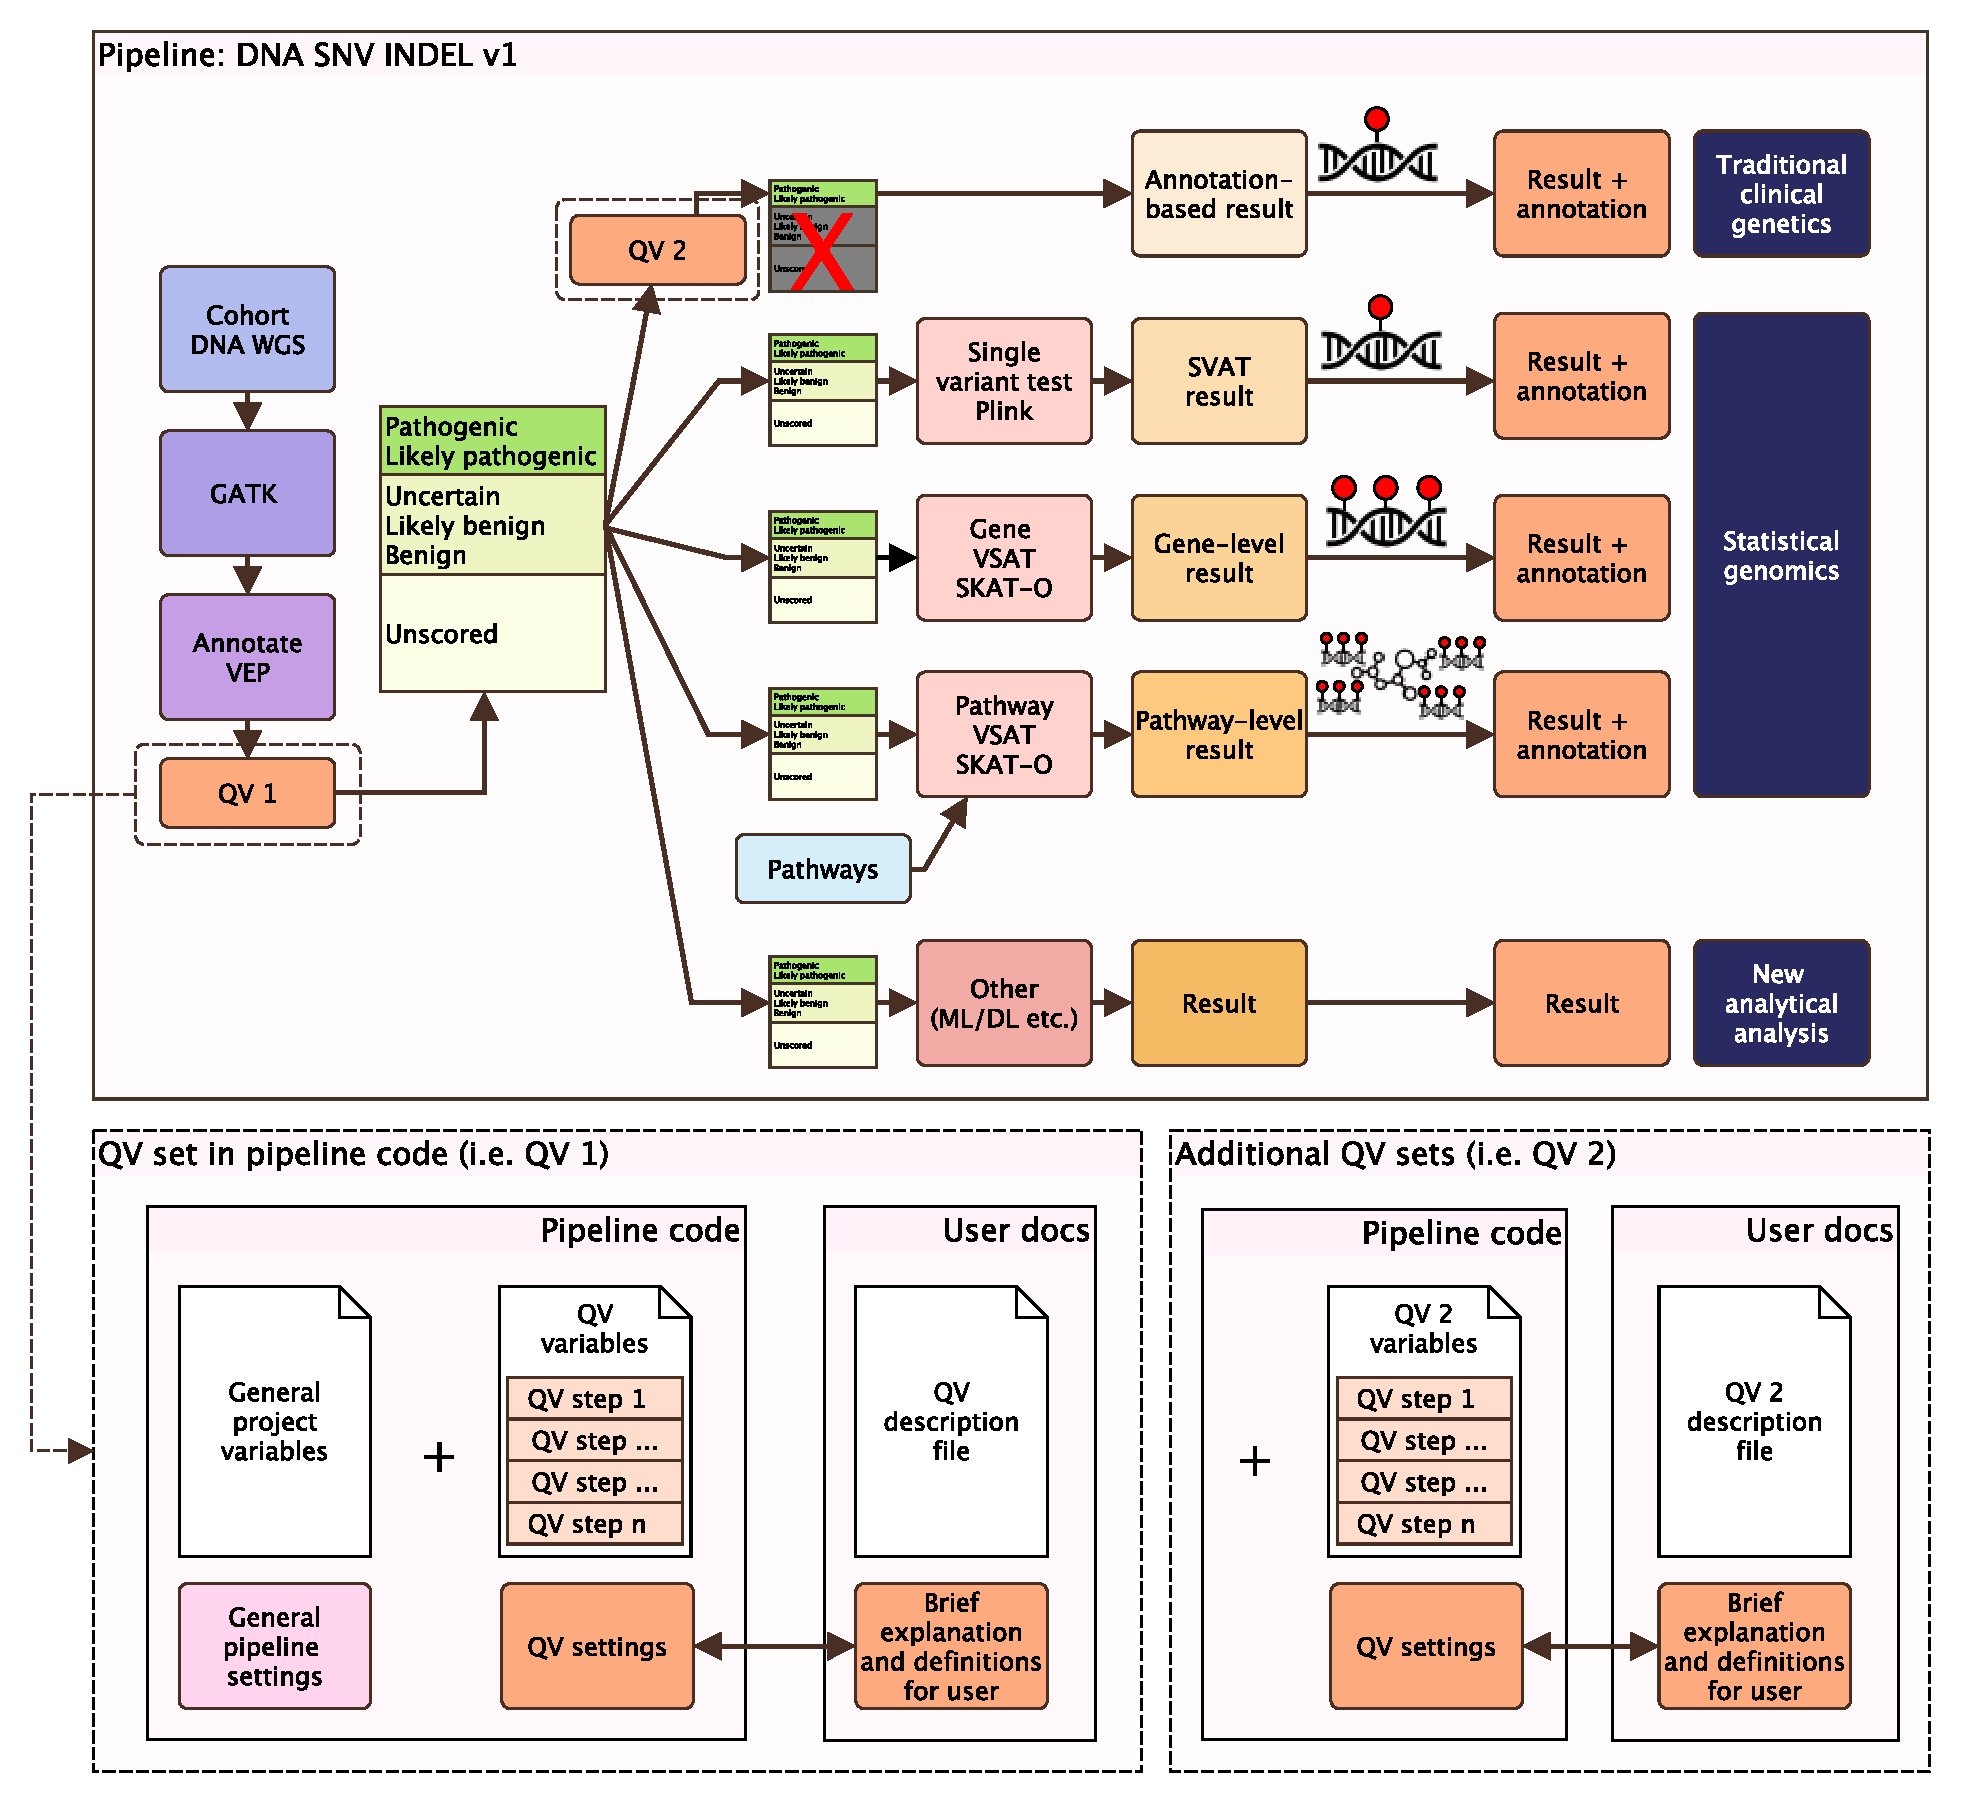
\includegraphics[width=0.99\textwidth]{./images/qv_pipeline_with_file_vcurrent.pdf}
    \caption{Summary of the example application design DNA SNV INDEL v1 pipeline. \ac{qv}1 and \ac{qv}2 are shown as sequential and potentially piped protocol steps.
    QV files used in a pipeline. The description file contains brief summary of how or why a step is used in the QV set (not mandatory). The variables file contains the necessary values of a QV setting (mandatory). These variables are loaded by the analysis pipeline. This illustration highlights a single stage in the QV1 set (i.e. step 10 in our example WGS analysis pipeline where the GATK VQSR method is applied). The full pipeline illustrated in the top panel simplifies this process under the QV1 icon.
    }
    \label{fig:qv_pipeline_with_file_vcurrent}
\end{figure}

The common approach to representing \ac{qv} steps are illustrated in 
\textbf{figure \ref{fig:qv_filter_pyramid_vcurrent}}.
This style simplifies the variant filtering process where each layer may arise from different stages of a pipeline.
The raw omic data can be processed into a multi-use analysis-ready format, as illustrated in 
\textbf{figure 
\ref{fig:candidate_variants_sequence_annotation}}.
Initial \ac{qv} steps can include \ac{qc} filtering. 
After variant annotation, further \ac{qv} steps can be applied on this new information as shown in 
\textbf{figure
\ref{fig:candidate_variants_sequence_annotation}}.
 
\begin{SCfigure}[][h]
%\begin{figure}[h]
\centering
     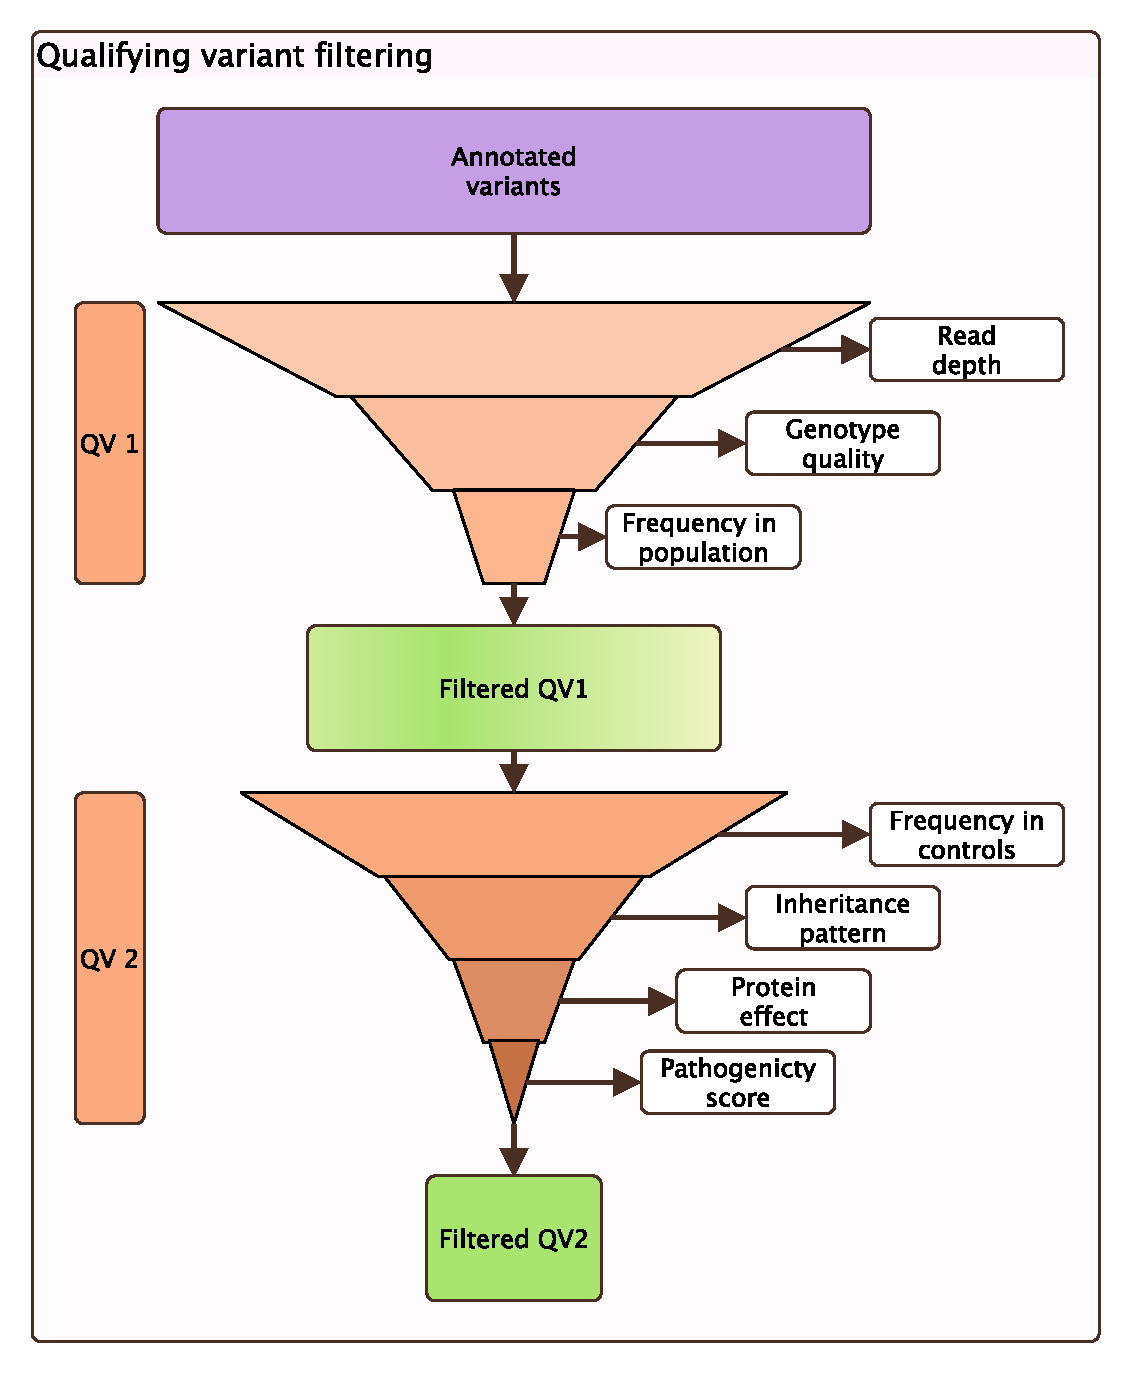
\includegraphics[width=0.66\textwidth]{./images/qv_filter_pyramid_vcurrent.pdf}
\caption{Illustration of the qualifying variant workflow. This figure summarises the conceptualised variant filtering step. This style is relatively common. In reality, we observe that each layer of the filters comes from disparate stages of a pipeline.}
    \label{fig:qv_filter_pyramid_vcurrent}
% \end{figure}
\end{SCfigure}

\citet{povysil2019rare} previously provided a tangible example of \ac{qv} for variant collapsing analyses for complex traits. 
\citet{cirulli2015exome} reported one of the first variant collapse analysis and introduced the \ac{qv} concept.
However, we have no a standardised framework for presenting \ac{qv} themselves. 
We detail four typical applications of \ac{qv} sets:

\begin{enumerate}
    \item \textbf{\ac{qv} passing \ac{qc} only}: Generates large datasets, e.g. 500,000 variants per subject, used in \ac{gwas} or \ac{wgs} pre-processing.
    \item \textbf{Flexible \ac{qv}}: Balances between \ac{qc} and false positives. For instance, fewer than 100,000 variants per subject in preparation for rare variant association testing.
        \item \textbf{\ac{qv}  for rare disease}: Produces smaller datasets after stringent filtering, e.g. 1,000 variants per subject, such as pre-processing to target known genes or a single causal variant in single-case genetic reports.
   \item \textbf{Known disease panel \ac{qv} set}: A well known gene panel with pathogenic variants, e.g. the \ac{acmg} \ac{sf} set, recommended for clinical reporting \cite{miller2023acmg}. 
   
\end{enumerate}

Two exemplary applications of \ac{qv}s are in clinical genetics reporting and \ac{gwas}. 
In clinical genetics single-case analysis, \ac{qv}s may be selected from a list of disease-causing genes identified by an expert panel. 
Variants within these genes can be categorised based on their potential pathogenicity into variants of unknown significance (VUS), or as known, candidate, or causal variants pending further analysis. 
In \ac{gwas}, \ac{qv}s generally refer to consensus variants that have undergone standard \ac{qc} procedures to ensure their statistical suitability for the main analysis.
The rigorous selection and categorisation of \ac{qv}s in genetic research and diagnostics are crucial for accurately reporting and reproducing such studies, underscoring the importance of \ac{qv} criteria, which can sometimes be more critical than the choice of analysis pipeline itself 
\cite{olson2023variant}.

\begin{figure}[h!]
    \centering
   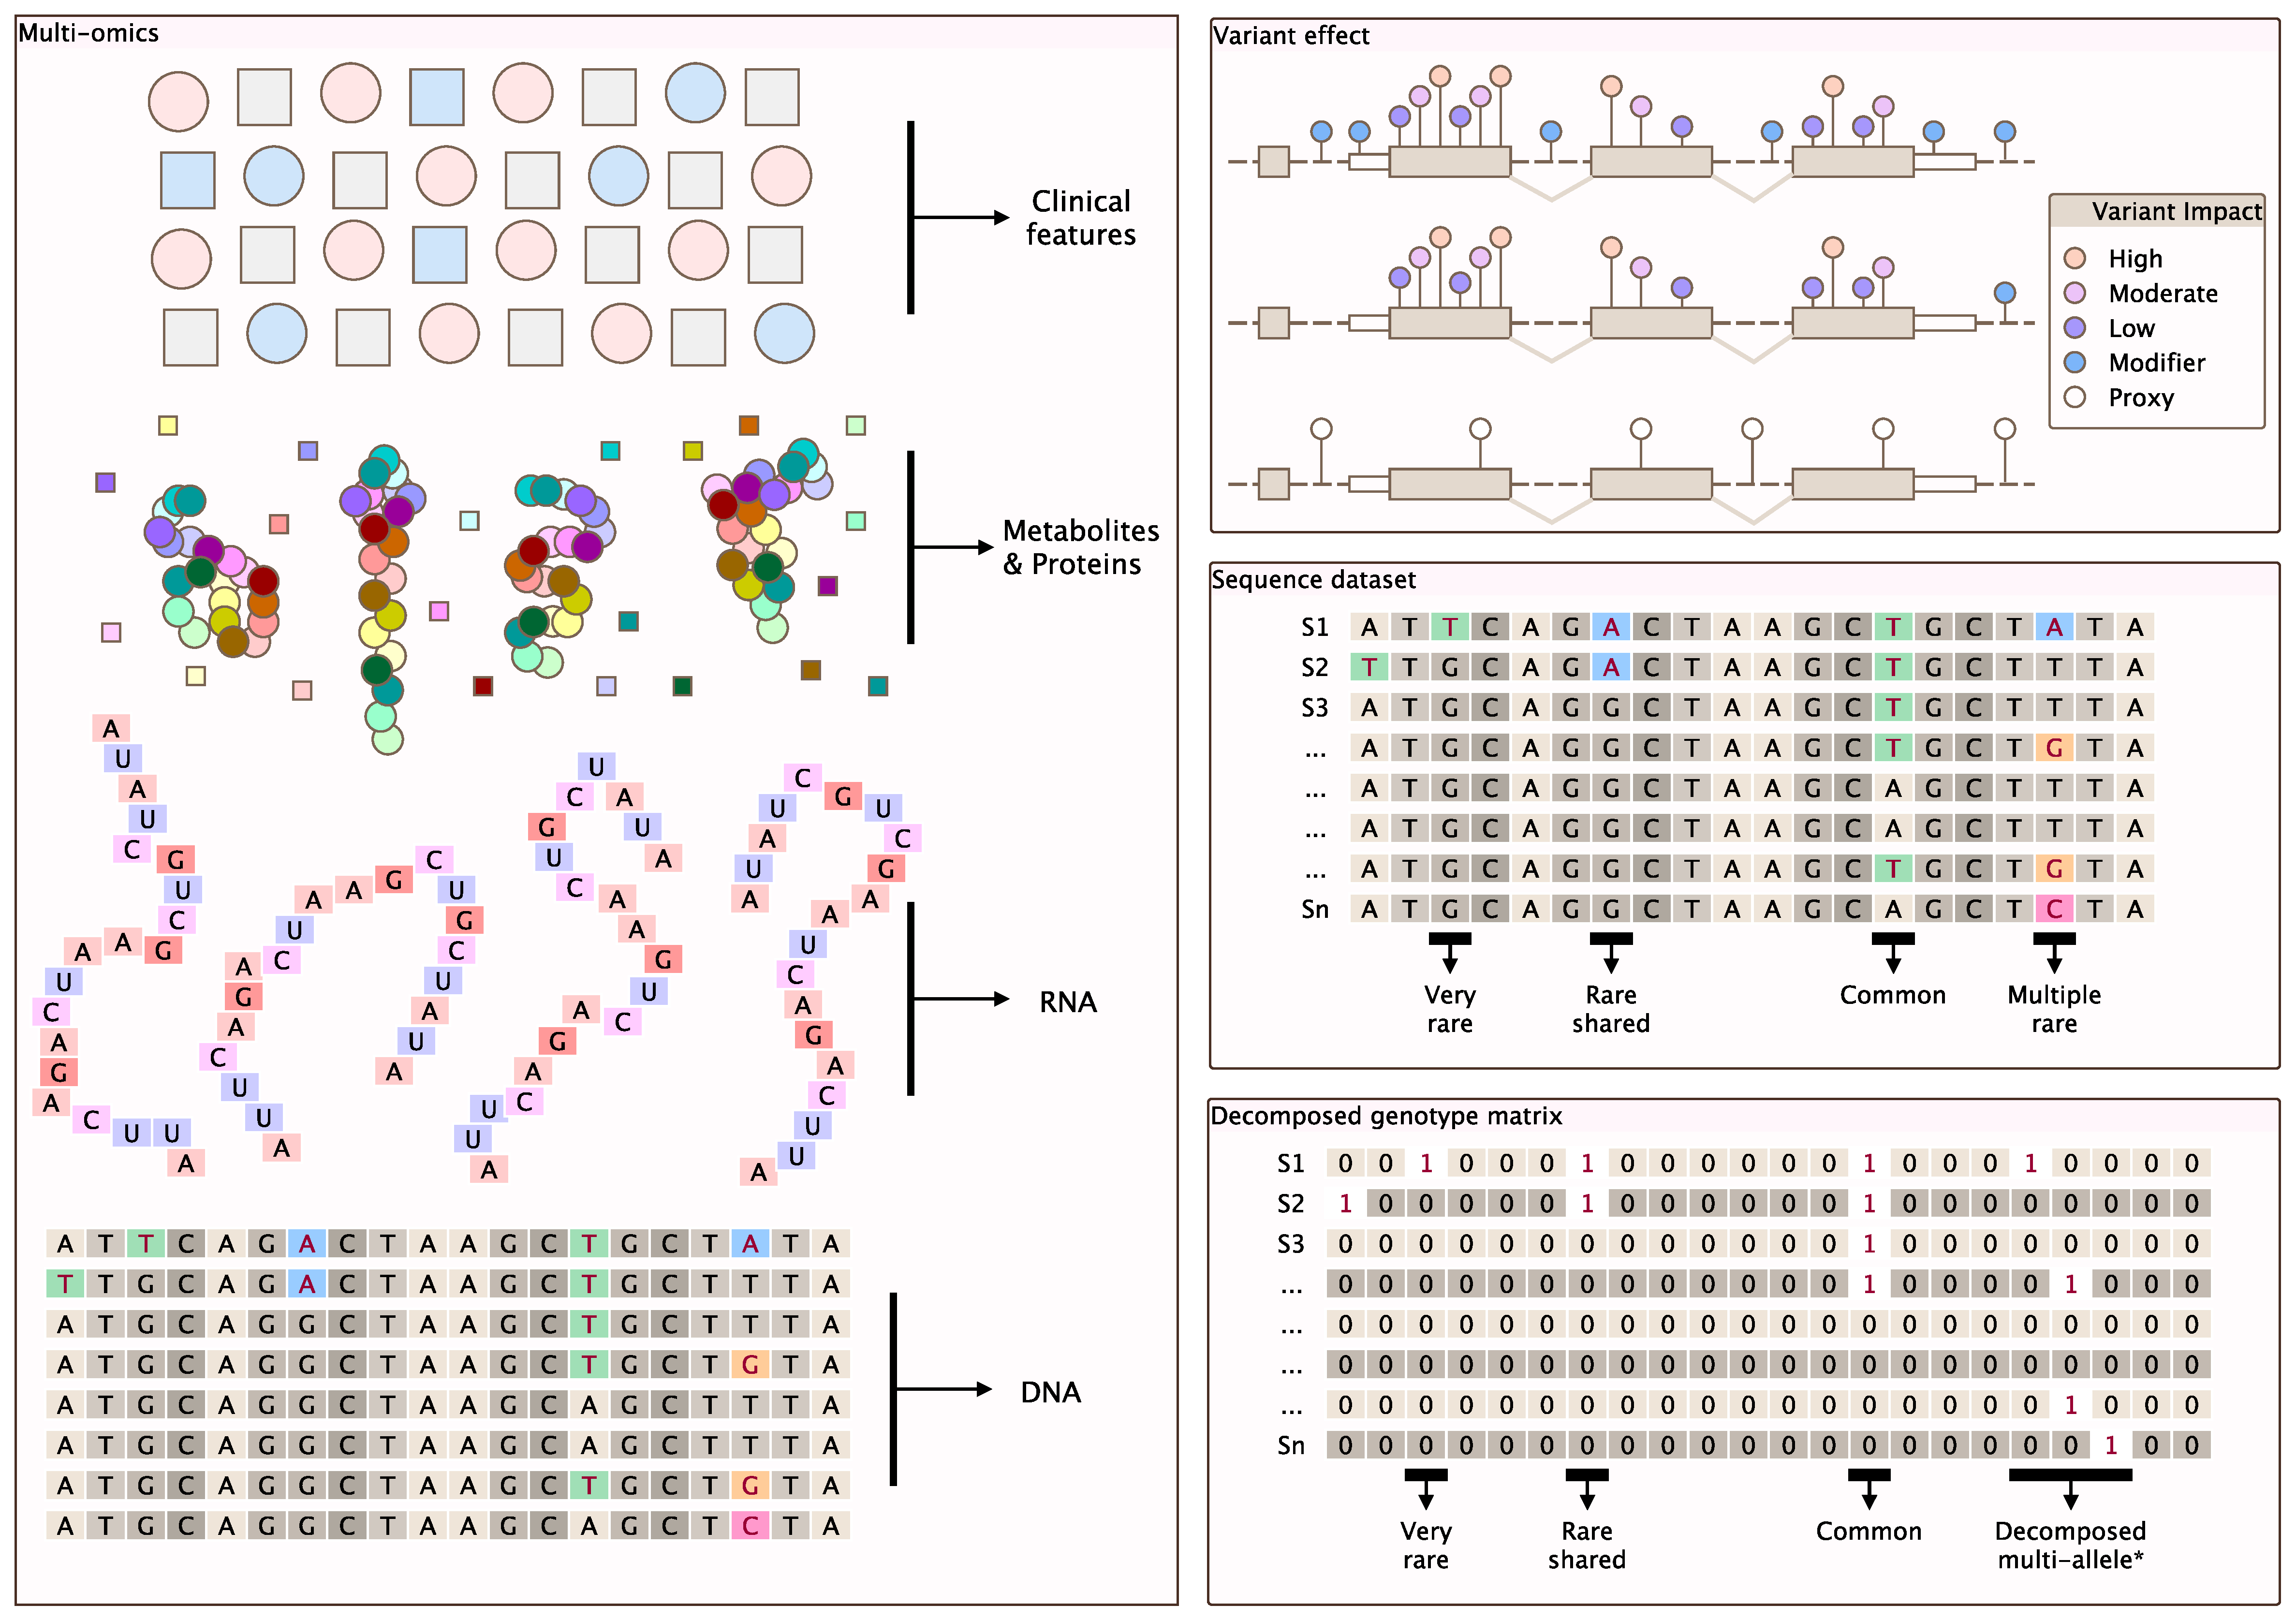
\includegraphics[width=0.8\textwidth]{./images/candidate_variants_sequence_to_matrix_pink.pdf}
      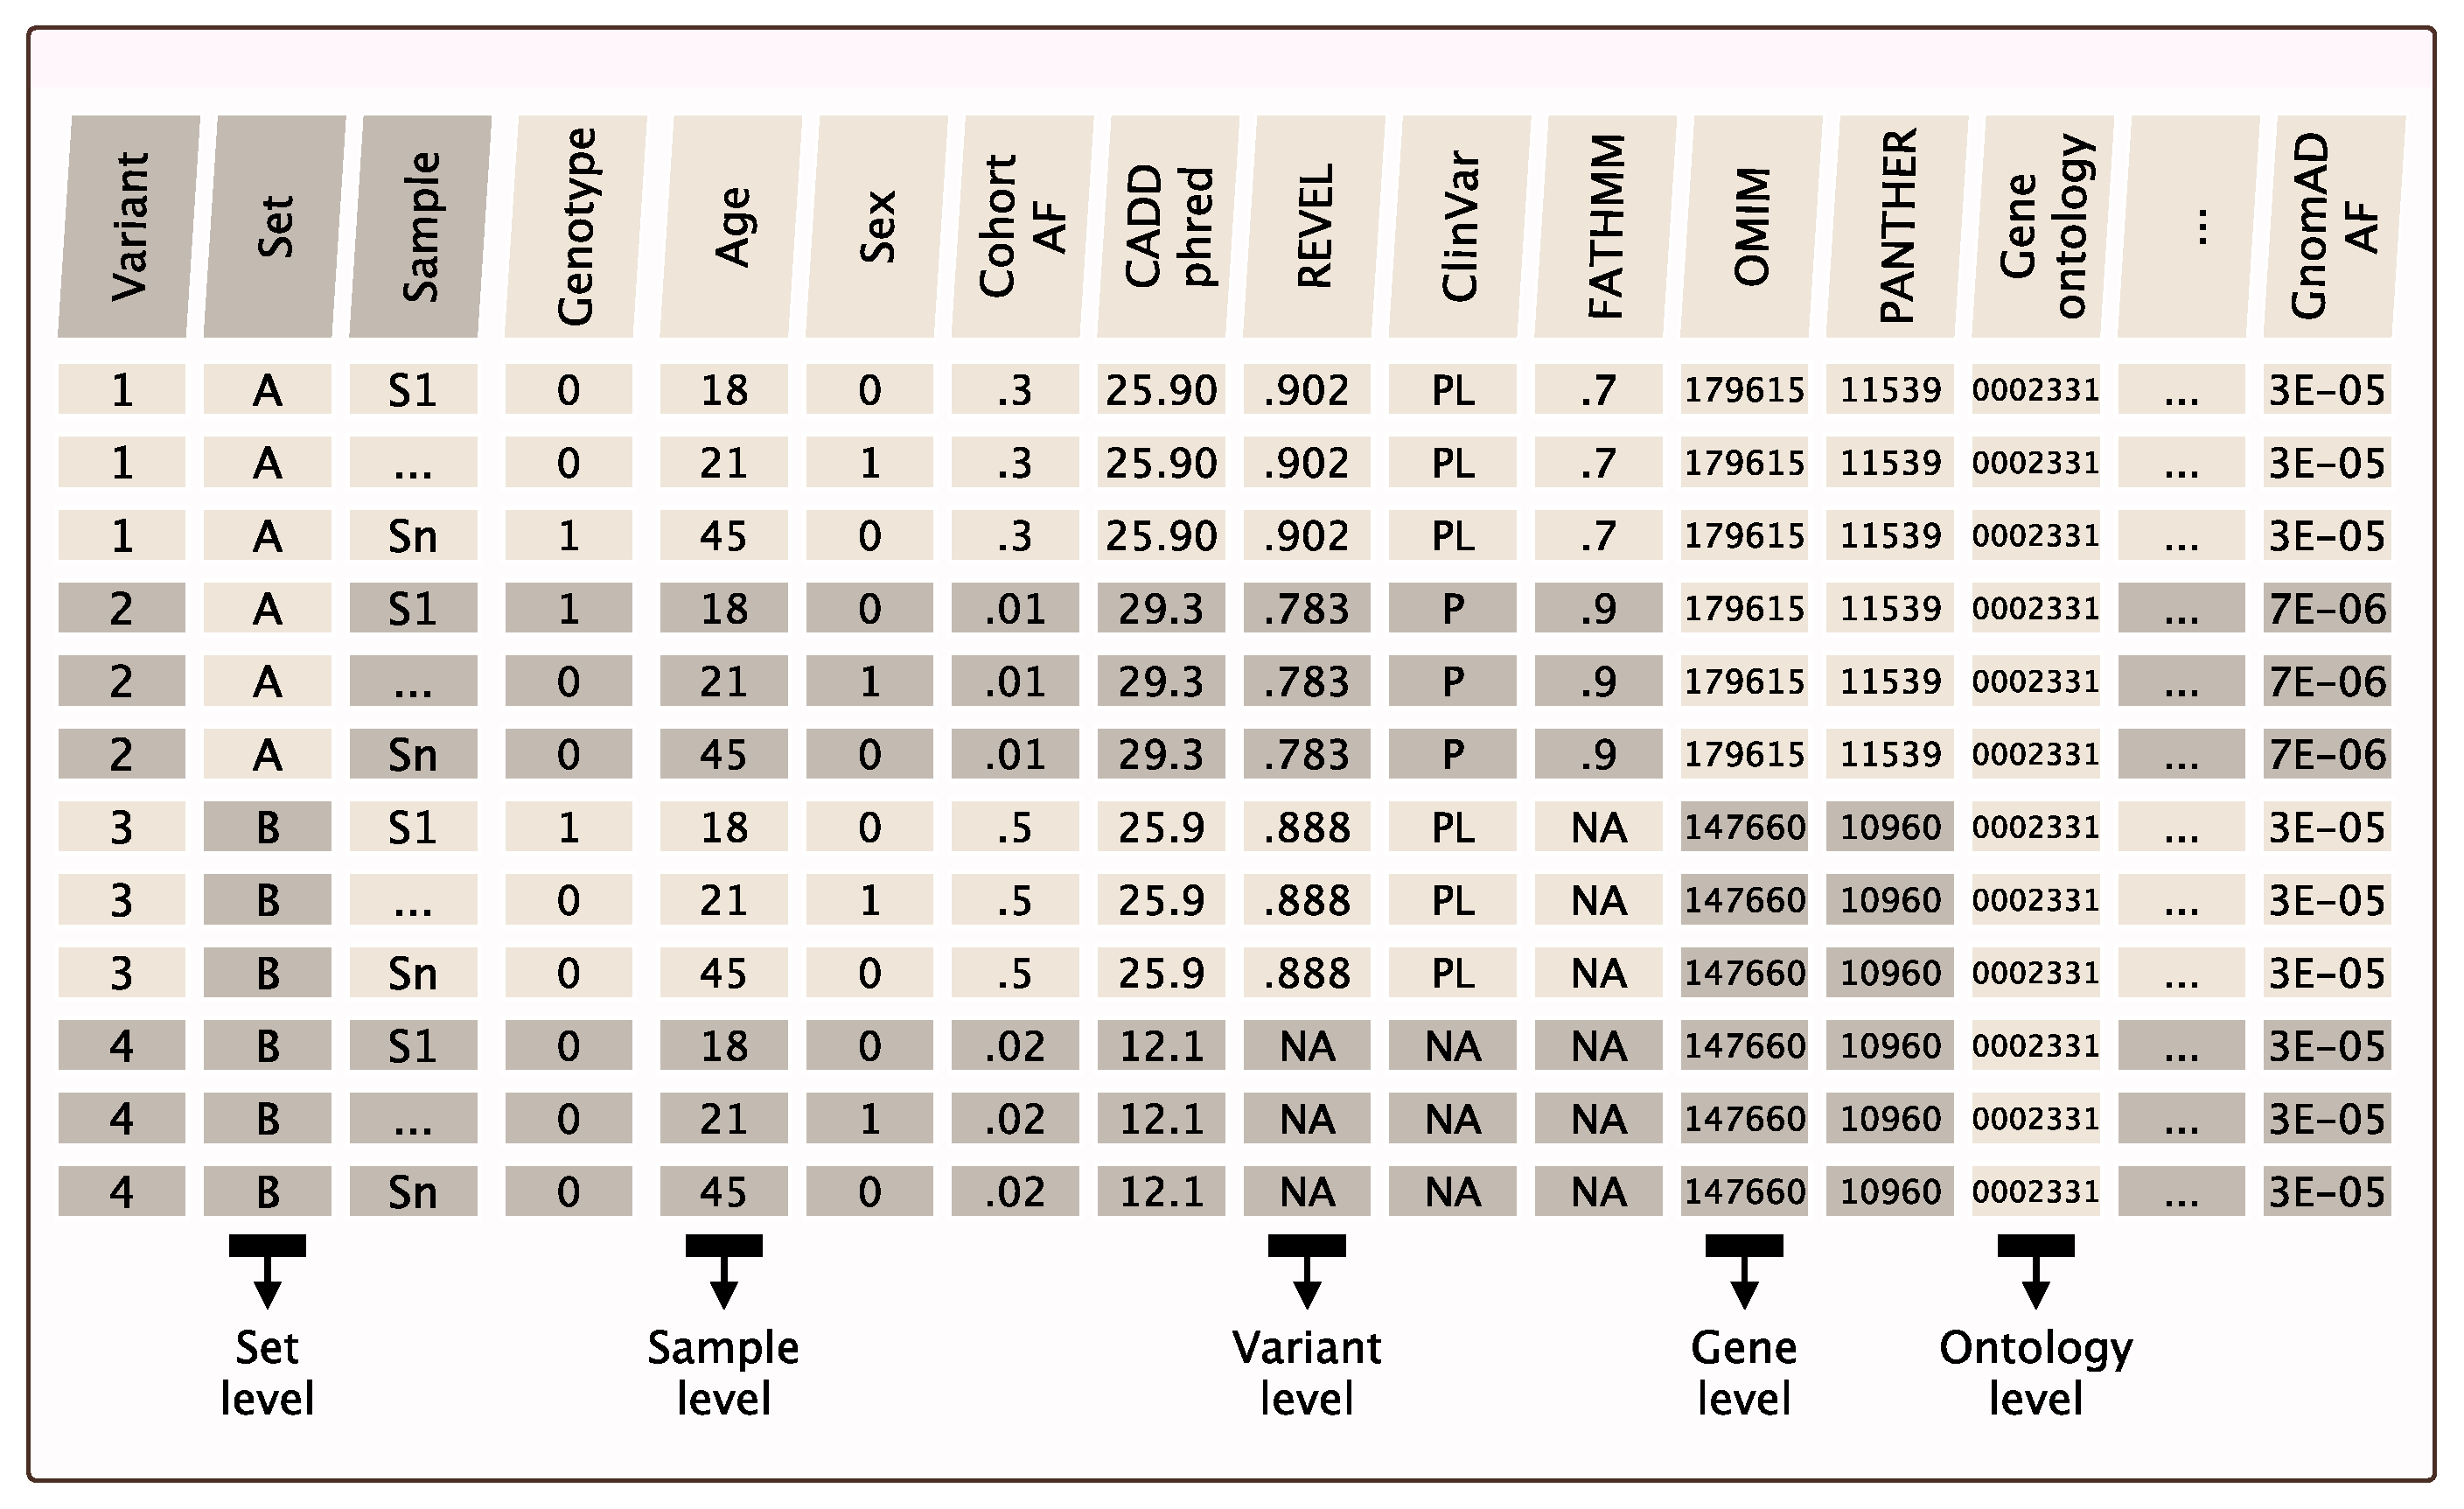
\includegraphics[width=0.8\textwidth]{./images/candidate_variants_sequence_annotation_pink.pdf}
    \caption{Top: From raw omics to data matrix.  We focus on DNA variants in \ac{qv} but the same concept applies to other datasets.
    Bottom: The initial variant detection pipeline generlly requires \ac{qc} and filtering rules that are the first \ac{qv} steps. Once complete, annotation of variants can follow. Further \ac{qv} steps can be run based on these new annotations.}
%    \label{fig:candidate_variants_sequence_to_matrix}
        \label{fig:candidate_variants_sequence_annotation}
\end{figure}

\section{Background problem and proposed solution}
%Historical context of \ac{qv}s and their evolution. Challenges faced in the qualification of variants and the necessity for standardisation.

As study sizes surpass the 1,000,000 subjects milestone \cite{lee2018gene, jansen2019genome}, the shift towards \ac{wgs} over genotyping has become standard. 
This transition enables the inclusion of rare variants in \ac{gwas} and \ac{vsat}, allowing for more comprehensive analyses of complex traits \cite{manolio2009finding, young2019solving}. % These paper describes the concept of ‘missing heritability’, the observation that heritability estimates from \ac{gwas} are much lower than those from twin studies.
\ac{qv} protocols are essential in data cleaning and preparation, serving as a critical step in ensuring the integrity of data analysis. 
While often grouped under the single term ``\ac{qv}'' for simplicity, the processes involved actually span various stages of a pipeline and originate from diverse steps or sources.
\textbf{Figure 
\ref{fig:qv_structure_vcurrent}}
shows the structural framework of a variant's features that may trigger specific \ac{qv} protocols, highlighting both pre-existing metadata and annotations added post-variant calling.

\begin{figure}[h!]
\centering
     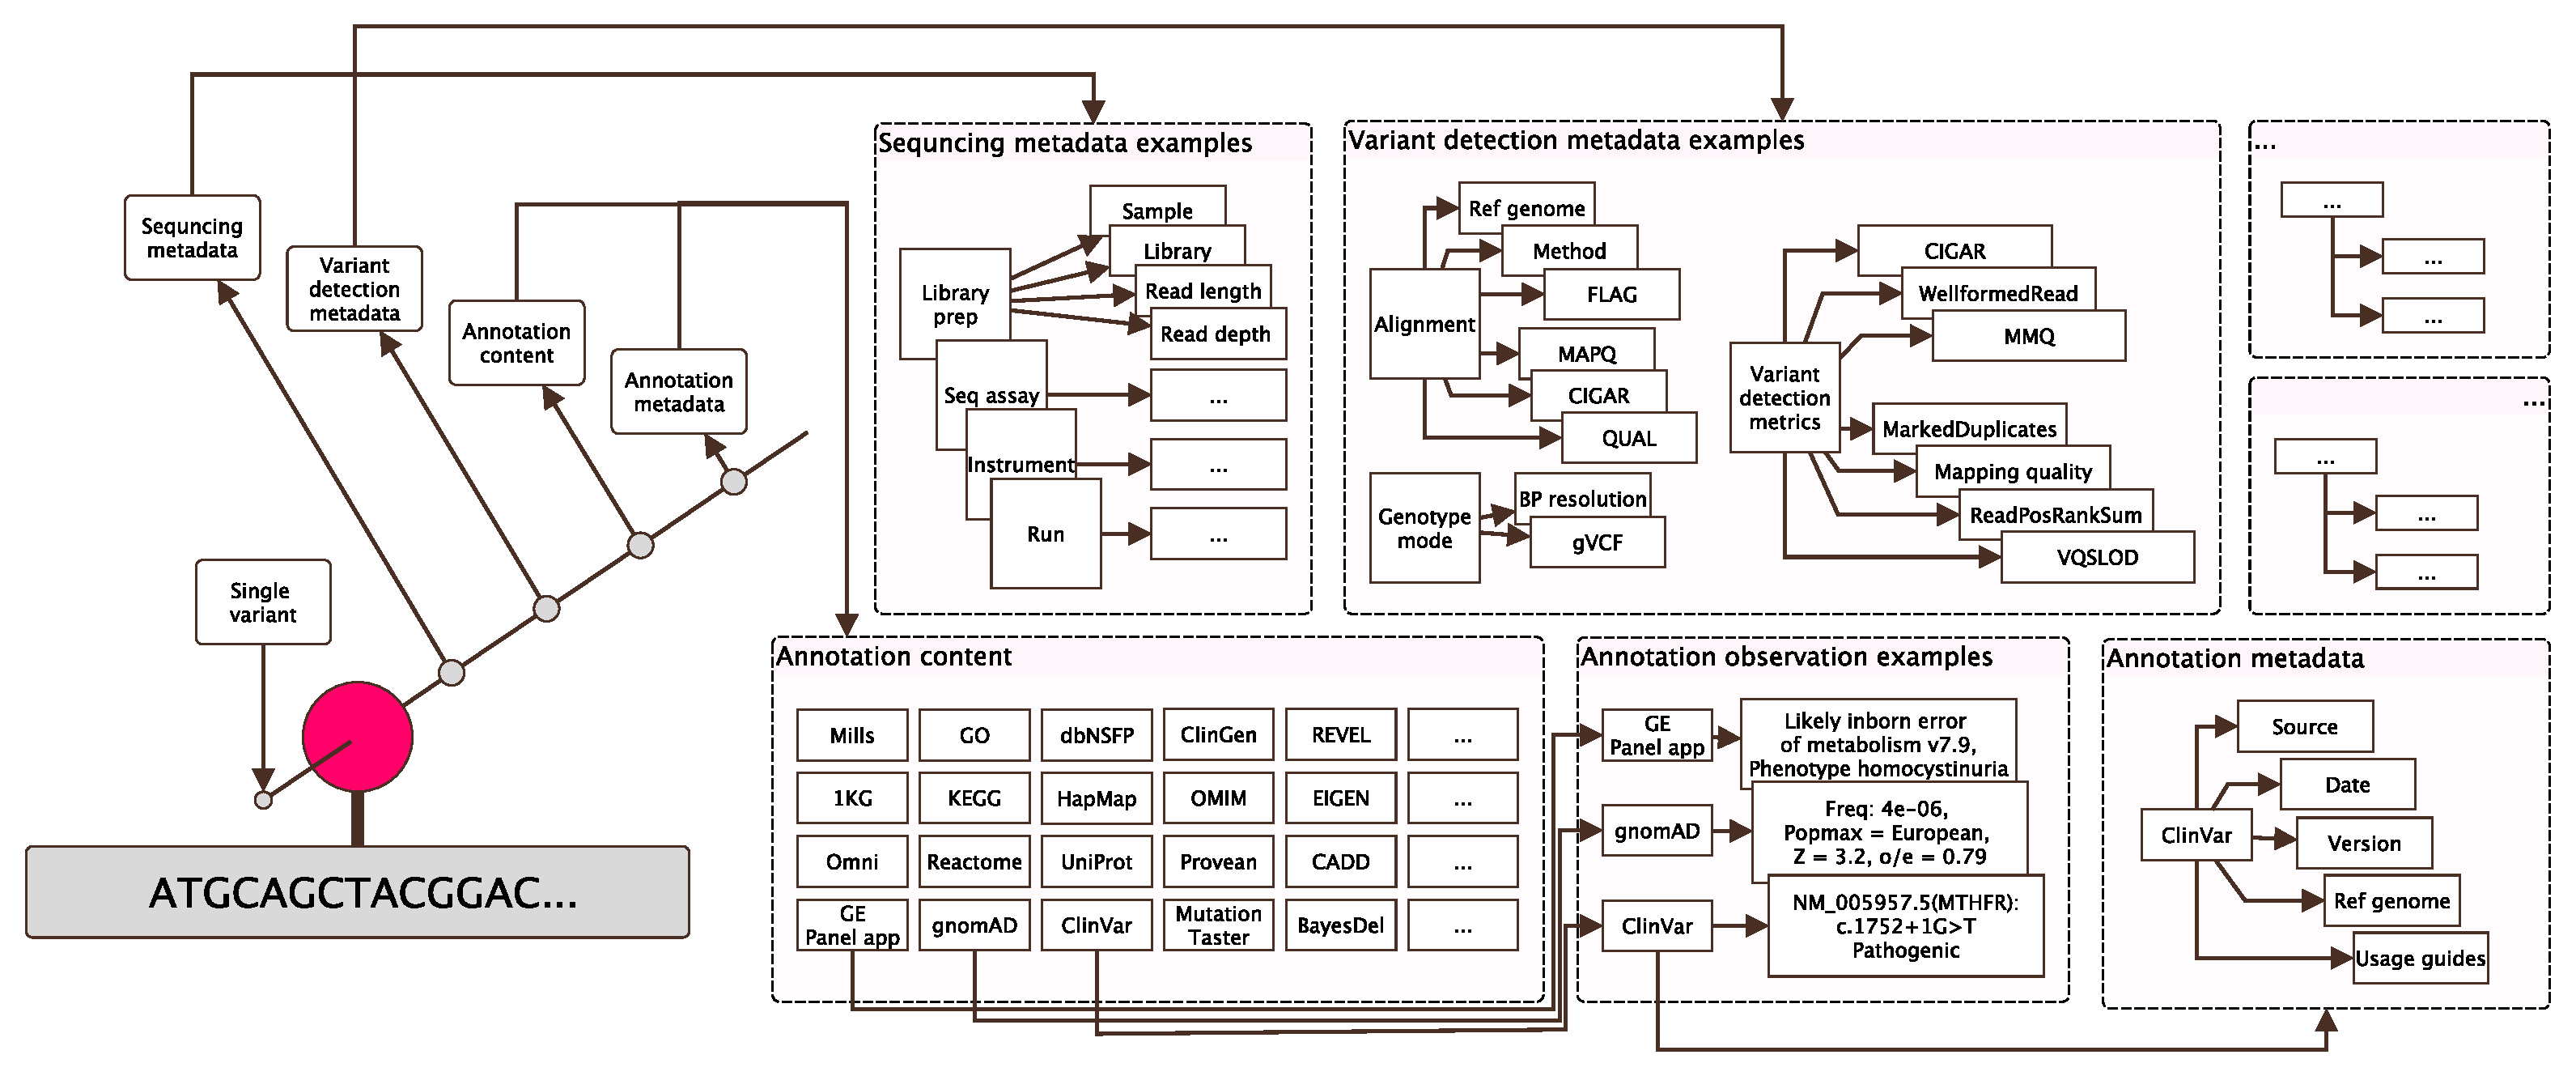
\includegraphics[width=0.99\textwidth]{./images/qv_structure_vcurrent.pdf}
\caption{This illustration shows the structural framework of an annotated variant in relation to the features used for qualification. For every individual variant, a number features are capable of triggering \ac{qv} protocols. The diagram highlights a select group of these features, showcasing both pre-existing metadata established before data generation and annotations applied after variant calling.}
\label{fig:qv_structure_vcurrent}
\end{figure}

Moreover, complex analyses often necessitate multiple processing streams that merge into a cohesive analysis. 
This multifaceted approach to \ac{qv} becomes apparent in multi-component analyses, which require the integration of two or more data sets. 
A standardised \ac{qv} format will allow for the use of various \ac{qv} sets, each based on potentially different filters and variables, yet provides a common foundation to ensure consistency and validity across disparate data streams

%\subsection{Challenges in Data Integration}
Unsurprisingly, the term \ac{qv} is often ambiguously used across different contexts within genomic studies, necessitating a clear definition for each application. 
Moreover, while \ac{qv}s are typically perceived as a set of filters and algorithms to remove benign or unrelated variants, they actually encompass many complex steps distributed throughout the entire analysis pipeline, and not necessarily confined to a single step. 
This dispersion of \ac{qv} steps challenges the conventional view and highlights the need for a flexible definition that not only encompasses their common uses but also acknowledges their implementation across multiple stages of genomic analysis.

The complex, multi-step nature of \ac{qv}s often goes unrecognised by those outside the field of bioinformatics.
This makes it challenging to share knowledge across disciplines for more advanced tasks and underscoring the importance of a clear and comprehensive understanding of \ac{qv} protocols.

By introducing a new vocabulary and a standard reference model for \ac{qv}s, we aim to clarify the concept and improve the communication and methodological discussions around \ac{qv}s. 
We therefore define and exemplify several common sets of \ac{qv}s, illustrating their potential configurations and roles within analysis pipelines:

\begin{enumerate}
    \item We demonstrate the theoretical pipelining of \ac{qv} sets.
    \item We outline how standardised \ac{qv} sets can be established for specific analytical scenarios.
    \item We highlight that \ac{qv}s are integral throughout the analysis pipeline, not merely as an end-stage addition but as essential components distributed across the process.
\end{enumerate}

Accordingly, the QV framework should furnish structured definitions that are both human and machine-readable to standardise the selection and interpretation of variants across diverse genomic studies. 
The methodology promotes efficient and precise variant detection and interpretation, which are essential for advancing both research and clinical diagnostics. 
Adhering to these structured analysis criteria aligns with the FAIR principles of findability, accessibility, interoperability, and reusability \cite{wilkinson2016fair}.

\section{Advanced applications and case study}
\subsection{How and why QV are used}
Here we provide an in-depth look at specific scenarios where \ac{qv}s  have inadvertently been crucial, such as in \ac{gwas}, \ac{wgs}, and clinical genetics. 
We note that application of \ac{qv}s would be appropriate in large-scale studies and rare disease research, such as sophisticated risk models that integrate clinical and genomic data, which enhance predictive accuracy in large, well-defined cohorts \cite{riveros2021integrated, weale2021validation, sun2021polygenic}.
% Thinking about complex models for clinical risk, such as PRS:
% \cite{riveros2021integrated} % This paper proposes a method to integrate clinical risk scores and PRSs for coronary artery disease and shows the improved predictive accuracy of PRSs over established clinical risk factors in European-ancestry individuals from the UK Biobank.
% \cite{weale2021validation} % This paper applies the integrated model proposed by Riveros-Mckay et al. (2021) to diverse populations in the UK Biobank and provides the first cross-ancestry validation of the clinical utility of adding polygenic scores into clinical risk tools.
% \cite{sun2021polygenic} % This paper recalibrated risk prediction models in the UK Biobank to what would be expected in an unbiased UK population to account for the bias caused by UK Biobank participants being healthier and wealthier, which is seldom considered in other studies in this field.
Likewise, \ac{qv} protocols can aid reproducibility across studies, especially in isolated or specific populations. This includes the analysis of complex signals within well-defined cohorts which can significantly aid rare disease studies \cite{lim2014distribution}. % This paper gives a good illustration of the value of isolated populations for identifying founder variants of large effect that are rare in other populations. We might consider a rare disease cohort in a similar way. 

\subsection{Example application of qualifying variants in WGS analysis}

Several \ac{qv} protocols can be piped together to create increasingly filtered datasets to match the needs at a certain stage of analysis. It is also typical that different analyses from \ac{qv}s sets are used and the final results from each step are merged to cover multiple scenarios. For example, a complex analysis pipeline might use all of
\colorbox{kispiblue!30}{\texttt{QV SNV/INDEL}} + 
\colorbox{kispiblue!30}{\texttt{QV CNV}} + 
\colorbox{kispiblue!30}{\texttt{QV structural variation}} + 
\colorbox{kispiblue!30}{\texttt{QV rare disease known}} + 
\colorbox{kispiblue!30}{\texttt{QV statistical association \ac{qc}}}, merged for a thorough multi-part analysis to reach the final combination of (1) a joint cohort disease association and (2) several single case analysis results.
We propose an example focusing on a SNV/INDEL pipeline using two \ac{qv} sets named 
\colorbox{colorSUNSET2!60}{\texttt{QV SNV INDEL v1}} and
\colorbox{colorSUNSET2!60}{\texttt{QV SNV INDEL v2}}.
The \ac{qv} sets are illustrated in 
\textbf{box \ref{box:pipe}}
and would be described in an analysis pipeline as follows:

%\begin{quotation}
``A cohort of patient WGS data was analysed to identify genetic determinants for the clinical diagnosis of phenotype X. 
This pipeline was concerned with WGS germline short variant discovery (SNVs + Indels) and interpretation.
\underline{First, a flexible \ac{qv} set (v1)} was used for cohort-level statistical genomics and \underline{second a rare disease \ac{qv} set (v2)} was used for single-case analysis.
(\textbf{1}) Data was processed with the 
\colorbox{colorSUNSET1!30}{\texttt{pipeline DNA SNV INDEL v1}} pipeline, which implements
(\textbf{a}) \colorbox{colorSUNSET2!60}{\texttt{QV SNV INDEL v1}} criteria, resulting in the prepared dataset
\colorbox{colorSUNSET3!30}{\texttt{dataset DNA SNV INDEL v1}}.
(\textbf{b}) The dataset was subsequently analysed in combination with other modules including 
\colorbox{colorSUNSET4!30}{\texttt{PCA SNV INDEL v1}} and 
\colorbox{colorSUNSET5!30}{\texttt{statistical genomics v1}} to complete statistical analysis on a joint cohort.
(\textbf{2}) Next, 
 the prepared dataset (from step 1a)
\colorbox{colorSUNSET3!30}{\texttt{Dataset DNA SNV INDEL v1}} was processed further with more strict filtering using
\colorbox{colorSUNSET2!60}{\texttt{QV SNV INDEL v2}} to identify previously known causal genetic variants for each patient based on disease-gene panel and curated evidence sources, resulting in \colorbox{colorSUNSET3!30}{\texttt{Dataset DNA SNV INDEL v2}} and final interpretation in
\colorbox{colorSUNSET5!30}{\texttt{single case report SNV INDEL v1}}.''
%\end{quotation}

\begin{tcolorbox}[
    % breakable,  % Allows the box to split over pages
    colback=white!0,  % No background color (fully transparent)
    colframe=black,  % Black border color
    boxrule=1pt,  % Width of the border
    arc=1mm,  % Radius of the corner rounding
    outer arc=1mm,
%    title=\textbf{Example diagrammatic representation}
   title=\textbf{\refstepcounter{myboxcounter}\label{box:pipe}Box \themyboxcounter: Example diagrammatic representation}
]

\dirtree{%
.1 \colorbox{colorSUNSET1!30}{\texttt{pipeline DNA SNV INDEL v1}}.
.2 Flexible \ac{qv} criteria.
.3 \colorbox{colorSUNSET2!60}{\texttt{QV SNV INDEL v1}} (-> \colorbox{colorSUNSET3!30}{\texttt{dataset DNA SNV INDEL v1}}).
.4 \colorbox{colorSUNSET4!30}{\texttt{PCA SNV INDEL v1}}.
.4 \colorbox{colorSUNSET5!30}{\texttt{statistical genomics v1}} -> Result 1.
.3 \colorbox{colorSUNSET3!30}{\texttt{dataset DNA SNV INDEL v1}}.
.4 Rare disease \ac{qv} criteria.
.5 \colorbox{colorSUNSET2!60}{\texttt{QV SNV INDEL v2}} (-> \colorbox{colorSUNSET3!30}{\texttt{dataset DNA SNV INDEL v2}}).
.6 \colorbox{colorSUNSET5!30}{\texttt{single case report SNV INDEL v1}} -> Result 2.
.3 Joint analysis output.
}

Joint analysis output from:\\
Result 1 = Cohort-level association signal (e.g. variant P-value). \\
Result 2 = Single variant for single patient.
\end{tcolorbox}


\section{Methodological framework}
\subsection{Three steps to a QV protocol}
We introduce 
a simple framework for the effective use of \ac{qv} protocols.
We use three steps to fulfil the needs of a pipeline as illustrated in 
\textbf{figure 
\ref{fig:qv_pipeline_with_file_vcurrent}}:
\begin{enumerate}
\item \textbf{Variables}: The criteria variables responsible which are sourced as part of a pipeline, as shown in \textbf{example box \ref{box:qv_variables_example}}.
\item \textbf{Description}: The description of each step as part of an overall \ac{qv} set, as shown in \textbf{example box \ref{box:qv_description_example}}.
\item \textbf{Source code}: The variables file can be sourced in pipeline code, as shown in \textbf{example box \ref{box:qv_bash_code_example}}.
\end{enumerate}

The practical application of our framework efficiently manages \ac{qv}-specific variables, such as \ac{af} thresholds, distinct from general pipeline settings. These variables can be imported and handled separately within the workflow to maintain clarity and specificity.  
We first provide a detailed example using \ac{vqsr} to show a full step in application of this method in a real-world genomic analysis scenario.
Later, we also illustrate this approach using workflow managers like Snakemake or Nextflow, demonstrating the separation and integration of these variables to streamline genomic processing tasks.

%Make a yed map to show the pipeline again, this time adding the explicit example of the VQSR variable settings from the variables.sh file.
%This show graphic summary icon for other \ac{qv} steps throughout the pipeline.
%Compare it to figure 1 where the summary of the pipeline simply illustrate \ac{qv} v1 as a single step but in this figure we see that it is actually spread throughout the pipeline by necessity. 

Individual steps in \ac{qv} criteria can have multiple types. 
For organisation in our protocols we suggest simple labels such as ``\ac{qc}'' and ``filter''. 
(1) Filtering thresholds such as \ac{af} (e.g. >0.1 in cohort, <0.1 in gnomAD). These might be directly applied in place to remove all affected variants. 
(2) Multiple steps with annotation labels such as \ac{qc} flags which do not remove variants but allow for downstream dissensions which which depend on multiple \ac{qv} criteria. 
Thus, in a \ac{qc} protocol a single step might run and filter all variants from criteria (1 ``filter'') and another filtering step might depend on several combined criteria (2 ``\ac{qc}'') which were added upstream.

\subsection{Detailed example QV variables}\label{sec:protocol_variables_example}
As a detailed example, we select the step \textbf{[\ac{qc}]} \colorbox{kispiblue!30}{\texttt{vqsr}} from the example \ac{qv} set
\colorbox{colorSUNSET2!60}{\texttt{QV SNV INDEL v1}}
to illustrate the variables sourced during the pipeline.
The following code snippet shows the from variables sourced during VQSR. 
First we set the mandatory \ac{qv} varaints in 
\textbf{box \ref{box:qv_variables_example}}.
Second, we provide the optional description in 
\textbf{box \ref{box:qv_description_example}}.
Third, we apply the variables in the source code 
\textbf{box \ref{box:qv_bash_code_example}}. 

\begin{tcolorbox}[
    breakable,  % Allows the box to split over pages
    colback=white!0,  % No background color (fully transparent)
    colframe=black,  % Black border color
    boxrule=1pt,  % Width of the border
    arc=1mm,  % Radius of the corner rounding
    outer arc=1mm,
%    title=\textbf{1. Example QV variables - extract from QV1 variables file}
     title=\textbf{\refstepcounter{myboxcounter}\label{box:qv_variables_example}Box \themyboxcounter: Example QV variables - extract from QV1 variables file}
]

\begin{verbatim}
# VQSR SNP Mode Variables
vqsr_snp_hapmap_known="false"
vqsr_snp_hapmap_training="true"
vqsr_snp_hapmap_truth="true"
vqsr_snp_hapmap_prior="15.0"

vqsr_snp_omni_known="false"
vqsr_snp_omni_training="true"
vqsr_snp_omni_truth="false"
vqsr_snp_omni_prior="12.0"

vqsr_snp_1000g_known="false"
vqsr_snp_1000g_training="true"
vqsr_snp_1000g_truth="false"
vqsr_snp_1000g_prior="10.0"

vqsr_snp_annotations="QD,MQ,MQRankSum,ReadPosRankSum,FS,SOR"
vqsr_snp_truth_sensitivity="99.7"

\end{verbatim}
\end{tcolorbox}

\begin{tcolorbox}[
    breakable,  % Allows the box to split over pages
    colback=white!0,  % No background color (fully transparent)
    colframe=black,  % Black border color
    boxrule=1pt,  % Width of the border
    arc=1mm,  % Radius of the corner rounding
    outer arc=1mm,
%    title=\textbf{2. }
         title=\textbf{\refstepcounter{myboxcounter}\label{box:qv_description_example}Box \themyboxcounter: Example QV description file (highlighting VQSR steps)}
]

\begin{enumerate}
    \item \textbf{[\ac{qc}]} \colorbox{kispiblue!30}{\texttt{fastp}} The tool fastp is used for ...
    \item \textbf{[\ac{qc}]} \colorbox{kispiblue!30}{\texttt{collectwgsmetrics}} BAMs that fail are ...
    \item \textbf{[\ac{qc}]} \colorbox{kispiblue!30}{\texttt{rmdup\_merge}} is used to mark ...
    \item \textbf{[\ac{qc}]} \colorbox{kispiblue!30}{\texttt{haplotype\_caller}} used \texttt{-ERC GVCF} mode for ...
    \item \textbf{[\ac{qc}]} \colorbox{kispiblue!30}{\texttt{\ac{qc}\_summary\_stats}} is used to log \ac{qc} ...
    \item \textbf{[\ac{qc}]} \colorbox{kispiblue!30}{\texttt{vqsr}} employs Variant Quality Score Recalibration (VQSR) using GATK. Includes the use of key metrics such as Quality by Depth (QD), Mapping Quality (MQ), and Read Position Rank Sum Test (ReadPosRankSum) to filter variants. The setting for SNPs are:
\begin{itemize}
    \item \textbf{VQSR SNP Mode - HapMap:} known=false, training=true, truth=true, prior=15.0. Used as a high-confidence reference set for training the recalibration model.
    \item \textbf{VQSR SNP Mode - Omni:} known=false, training=true, truth=false, prior=12.0. Provides additional training data derived from Omni genotyping arrays.
    \item \textbf{VQSR SNP Mode - 1000G:} known=false, training=true, truth=false, prior=10.0. Utilizes data from the 1000 Genomes Project to inform the model on common SNP variations.
    \item \textbf{VQSR Annotations - QD, MQ, MQRankSum, ReadPosRankSum, FS, SOR:} Annotations are metrics used to predict the likelihood of a variant being a true genetic variation versus a sequencing artifact. They include quality by depth, mapping quality, mapping quality rank sum test, read position rank sum test, Fisher's exact test for strand bias, and symmetric odds ratio of strand bias.
    \item \textbf{VQSR Truth Sensitivity Filter Level:} 99.7. Specifies the percentage of true variants to retain at a given VQSLOD score threshold, set here to capture 99.7\% of true variants.
    \end{itemize}    
\end{enumerate}
\end{tcolorbox}

\begin{tcolorbox}[
    breakable,  % Allows the box to split over pages
    colback=white!0,  % No background color (fully transparent)
    colframe=black,  % Black border color
    boxrule=1pt,  % Width of the border
    arc=1mm,  % Radius of the corner rounding
    outer arc=1mm,
%    title=\textbf{3. Example code sourcing the variables file}
    title=\textbf{\refstepcounter{myboxcounter}\label{box:qv_bash_code_example}Box \themyboxcounter: Example code sourcing the variables file}
]

\lstinputlisting{example_qv_code.sh}
\end{tcolorbox}

\subsection{Simple example with a workflow manager}
We demonstrate the use of a \ac{qv} variable file within a workflow manager, such as Snakemake or Nextflow
(\textbf{box \ref{box:qv_variables_example_workflow1}}).
The setup involves two types of YAML configuration files: one for general pipeline settings and another specifically for \ac{qv}-related variables
(\textbf{box \ref{box:qv_variables_example_workflow2}}).
These configurations are integrated into the primary analysis script, typically a Snakefile, ensuring that all parameters required for genomic analyses are systematically managed and applied 
(\textbf{box \ref{box:qv_variables_example_workflow3}}). 

\begin{tcolorbox}[
    breakable,  % Allows the box to split over pages
    colback=white!0,  % No background color (fully transparent)
    colframe=black,  % Black border color
    boxrule=1pt,  % Width of the border
    arc=1mm,  % Radius of the corner rounding
    outer arc=1mm,
%    title=\textbf{1. Example QV variables - extract from QV1 variables file}
     title=\textbf{\refstepcounter{myboxcounter}\label{box:qv_variables_example_workflow1}Box \themyboxcounter: Example worflow manager - yaml}
]

\begin{verbatim}
# qv_config.yaml
min_depth: 10
max_allele_frequency: 0.01
quality_score_threshold: 20
\end{verbatim}
\end{tcolorbox}

\begin{tcolorbox}[
    breakable,  % Allows the box to split over pages
    colback=white!0,  % No background color (fully transparent)
    colframe=black,  % Black border color
    boxrule=1pt,  % Width of the border
    arc=1mm,  % Radius of the corner rounding
    outer arc=1mm,
%    title=\textbf{1. Example QV variables - extract from QV1 variables file}
     title=\textbf{\refstepcounter{myboxcounter}\label{box:qv_variables_example_workflow2}Box \themyboxcounter: Example worflow manager - yaml}
]
\begin{verbatim}
# config.yaml
reference_genome: "path/to/reference/genome.fasta"
annotation_file: "path/to/annotation.gtf"
sample_list: "path/to/samples.txt"
output_dir: "path/to/output"
qv_config: "qv_config.yaml"
\end{verbatim}
\end{tcolorbox}



\begin{tcolorbox}[
    breakable,  % Allows the box to split over pages
    colback=white!0,  % No background color (fully transparent)
    colframe=black,  % Black border color
    boxrule=1pt,  % Width of the border
    arc=1mm,  % Radius of the corner rounding
    outer arc=1mm,
%    title=\textbf{1. Example QV variables - extract from QV1 variables file}
     title=\textbf{\refstepcounter{myboxcounter}\label{box:qv_variables_example_workflow3}Box \themyboxcounter: Example worflow manager - python}
]
\begin{verbatim}
# Snakefile
configfile: "config.yaml"
qv_settings = read_yaml(config["qv_config"])

rule all:
  input:
    "results/filtered_variants.vcf"

rule filter_variants:
  input:
    "data/raw_variants.vcf"
  output:
    "results/filtered_variants.vcf"
  params:
    depth = qv_settings['min_depth'],
    af = qv_settings['max_allele_frequency'],
    qs = qv_settings['quality_score_threshold']
  shell:
    """
    bcftools filter -i 'DP>{depth} && AF<{af} && \
    QUAL>{qs}' {input} > {output}
    ""
\end{verbatim}
\end{tcolorbox}

\section{Examples of real-world QV applications}

\subsection{Discovery research}
\citet{greene2023genetic} developed what can effectively be considered a prime example of QV standardisation with their ``Rareservoir,'' a relational database schema optimised for handling genetic data from rare disease studies.
This database optimises storage and query speed by focusing on rare variants - those with a \ac{maf} below 0.1\% - thus reducing data size by about 99\%. Variants are stored as 64-bit integers (``RSVR IDs''), organised by genomic position to support efficient location-based queries. 
Additional data include \ac{maf}s from gnomAD, CADD pathogenicity scores, and impact predictions per the Sequence Ontology. Genetic impacts are encoded into a 64-bit integer (``CSQ ID''), where each bit corresponds to a specific gene function impact, ranked by severity. 
This structure enables precise database queries. 
By employing the Bayesian genetic association method BeviMed, initially described by \citet{greene2017fast}, the study effectively inferred associations between genes and rare disease phenotypes, demonstrating the capacity to handle and analyze complex genetic datasets effectively.
 The protocol by \citet{greene2023genetic} can be produced in the QV format, easing the interpretation and reproducibility.

We are applying the \ac{qv} framework in ``SwissPedHealth''. 
This is a joint paediatric national data stream where one of the objectives is to investigate rare/unknown disease using a multiomic approach, including \ac{wgs}, RNAseq, proteomics, and clinical data
\cite{mozun2024paediatric}.
We optimise the processing pipelines by using consensus raw datasets (e.g. WGS in patients and families), which is annotated and filtered to several \ac{qv} levels.
The resulting pre-processed datasets are suitable for a range of analysis including \ac{gwas}, \ac{vsat}, single-case clinical genetics reports, machine learning, and joint multiomic analysis. 

National-scale projects reuse data many times and naturally require the use of \ac{qv}, currently in the traditional format; mixed throughout pipelines without explicit distinction.
The  Genomics England 100,000 Genomes Project performs central automated analysis with interpretation and clinical reporting \cite{turnbull2018100}. 
This data is then used in many subsequent research projects. 
One significant application of \ac{qv} protocols is in genomics-based newborn screening, which has been gaining traction as a pivotal healthcare innovation
\cite{noauthor_every_2024}. 

\subsection{Rapid diagnostics}
% WGS diagnostic
Screening for known disease is by default, based on searching for a known \ac{qv} set. 
The use of a formalised standard would allow for consistency and reliability for stakeholders. 
Genome analysis in neurodevelopmental disorders in 465 families found causal variants in 36\% of 489 affected individuals \citep{sanchis2023genome}.
The DDD study involved over 13,500 families; approximately 41\% of probands received a genetic diagnosis \cite{wright2023genomic}.
Genomic lifespan association in Iceland was reported by \citet{jensson2023actionable}, which included 57,933 participants, identifying 2,306 individuals with actionable genotypes linked to a decrease in median lifespan by approximately three years for carriers.

% speed
We propose that the use of standardised \ac{qv} can aid in developing rapid genomic diagnostics. 
In UAE, rapid whole-genome sequencing - \citep{abou2023rapid}
allowed for rapid whole-genome sequencing with a turnaround of 37 hours on average.
\citet{meng2017use} reported on 278 critically ill infants; molecular diagnosis achieved in 36.7\% of cases, with higher rates (50.8\%) in critical trio exome cases. They reported an impacted medical management in 52.0\% of diagnosed cases.
\citet{lunke2023integrated} reported in the national scale multi-omics for rare diseases, involving 290 critically ill infants and children; diagnostic yield from WGS initially at 47\%, increased to 54\% with extended analysis.
Altered critical care  management occurred for 77\% of diagnosed cases.

\subsection{Complex variant calls}
% other types of analysis
Additionally, using the \ac{qv} framework for different analysis types, such as SNV-INDEL, copy-number variants, and structural variants, means that simple \ac{qv} IDs can be used for database reporting. 
Researchers can then easily query whether or not additional analysis is expected to reveal more findings. 
For instance,
\citet{wojcik2024genome} used genome sequencing in 822 families with rare monogenic diseases, achieving a diagnostic yield of 29.3\%.
They focused on broader genomic coverage including structural and non-coding variants, identifying causative variants in 8.2\% of cases previously undetected by exome sequencing.

\subsection{Secondary findings}
\label{sec:sf}
The \ac{acmg} \ac{sf} v3.2 list, exemplifies a well-defined and impactful application of \ac{qv} standards in genomic medicine 
\cite{miller2023acmg}. 
This list specifies gene-phenotype pairs recommended for reporting as secondary findings during clinical exome and genome sequencing. 
Such standardisation not only streamlines the identification of clinically actionable genetic information but also enhances the consistency and quality of genomic data interpretation across different settings.
The key limitation is that this dataset is relatively unstructured meaning that each implementation requires extensive work and care on the part of front-line analysts. 
The \ac{acmg} \ac{sf} list is revised annually, reflecting its dynamic nature and the evolving understanding of gene-disease correlations. 
Each version, such as the current v3.2, includes detailed criteria for the inclusion or exclusion of specific genes, based on rigorous evidence of their association with significant health outcomes. 
This methodical approach to curating the \ac{sf}  list ensures that it remains a reliable resource for opportunistic screening in a clinical context.

\textbf{Table \ref{tab:transposed_acmg_sf_list}} lists the first two entries (transposed) from the \ac{acmg} \ac{sf} list showcasing specific genes associated with cardiovascular phenotypes.
We then represent this data in a standardised \ac{qv} format in
\textbf{box
\ref{box:qv_variables_example_sf} - 
\ref{box:qv_variables_example_sf2}},
which can be used in any variant filtering program as demonstrated.
In bioinformatics pipelines, specifying \ac{qv} sets consistently, such as \ac{acmg} \ac{sf} v3.2 allows patients to receive the most relevant and up-to-date information regarding their genetic health risks, without missing out on simple checks due to the burden of manually implementing new \ac{qv}. 

\begin{table}[ht]
\centering
\caption{The first two entries from the ACMG SF v3.2 list, transposed, for reporting of secondary findings in clinical exome and genome sequencing \cite{miller2023acmg}.}
\begin{tabular}{@{}lp{4.5cm}p{4.5cm}@{}}
\toprule
\textbf{Detail}             & \textbf{ACTA2}                      & \textbf{ACTC1} \\
\midrule
Disease/Phenotype           & Familial thoracic aortic aneurysm   & Hypertrophic cardiomyopathy \\
Gene MIM                    & 102620                              & 102540 \\
Disorder MIM                & 611788                              & 612098 \\
Phenotype Category          & Cardiovascular                      & Cardiovascular \\
Inheritance                 & AD                                  & AD \\
Variants to report          & All P and LP                        & All P and LP \\
\bottomrule
\end{tabular}
\label{tab:transposed_acmg_sf_list}
\end{table}

\begin{tcolorbox}[
    breakable,  % Allows the box to split over pages
    colback=white!0,  % No background color (fully transparent)
    colframe=black,  % Black border color
    boxrule=1pt,  % Width of the border
    arc=1mm,  % Radius of the corner rounding
    outer arc=1mm,
    title=\textbf{\refstepcounter{myboxcounter}\label{box:qv_variables_example_sf}Box \themyboxcounter: QV configuration for SF - yaml}
]
\begin{verbatim}
# qv_sf_v3.2_config.yaml
genes:
- gene: "ACTA2"
   inheritance_pattern: "AD"
   variant_class : ["Pathogenic", "Likely Pathogenic"]
- gene: "ACTC1"
   inheritance_pattern: "AD"
   variant_class: ["Pathogenic", "Likely Pathogenic"]
...
\end{verbatim}
\end{tcolorbox}

\begin{tcolorbox}[
    breakable,  % Allows the box to split over pages
    colback=white!0,  % No background color (fully transparent)
    colframe=black,  % Black border color
    boxrule=1pt,  % Width of the border
    arc=1mm,  % Radius of the corner rounding
    outer arc=1mm,
    title=\textbf{\refstepcounter{myboxcounter}\label{box:qv_variables_example_sf2}Box \themyboxcounter: Filtering command for QV SF}
]
\begin{verbatim}
# Pseudo-code to filter variants for each gene 
# in ACMG SF v3.2 list:

Read genes from qv_sf_v3.2_config.yaml

For each gene entry in genes:
  Apply filter command:
    filter -i 'GENE=="{gene['gene']}" && 
    INHERITANCE=="{gene['inheritance_pattern']}" && 
    (VARIANT_CLASSIFICATION in gene['variant_class'])' 
    input.vcf > output_{gene['gene']}_qv_sf.vcf
\end{verbatim}
\end{tcolorbox}

\section{Alignment with patient and public involvement needs}
A key benefit of our framework is that it provides explicit citable documentation of which genetic variants are included or excluded in a database or report. 
This transparency allows both analysts and patients to clearly see how filtering is performed, thereby bolstering trust and facilitating meaningful patient and public involvement (PPI). 
For example, as illustrated in 
\textbf{section \ref{sec:sf}}
 both the analyst and the patient can confirm that the \ac{acmg} clinical guidelines on \ac{sf} have been applied. 
This ensures that important findings-such as ruling out false negatives like ``no known causes of hereditary breast and/or ovarian cancer''-are not overlooked, ultimately enhancing patient care and informed decision-making.

\section{Challenges and innovations}
\subsection{Avoiding pitfalls}
% Analysis of pitfalls similar to those in repeated measures analysis (Bland \& Altman reference). Addressing Simpson's paradox and path analysis in the context of multi-omic data integration. Application of advanced statistical frameworks for source-specific variations.
In the pursuit of advancing omics research through multiblock data, we recognize the imperative need to standardise and optimise the use of \ac{qv}. 
This need mirrors the simple pitfalls in the analysis of repeated measures, where combining repeated measurements without appropriate controls can lead to misleading conclusions
\cite{bland1994correlation}.
So we must approach the integration of complex \ac{qv} layers with rigor.

In multi-omic integration, where data from various layers such as DNA, RNA, and protein are fused, the naive merging of data without considering the unique source and nature of each data block can similarly mislead. 
The warning from \citet{bland1994correlation} about repeat data, or Simpson's paradox, where aggregated data can obscure real relationships, underscore the necessity for sophisticated statistical frameworks that acknowledge and adjust for the intricacies of source-specific variations.
Once acknowledged, these features can be addressed potentially with existing methods
\cite{simpson1951interpretation, wright1934method, pearl2016causal}.
% Notably, Pearl et al. (2016) assert that they can “fully resolve Simpson’s Paradox by determining which variables to measure and how to estimate causal effects under confounding” (p. 44). 
Increasingly deep phenotyping and precision medicine with omic data are reshaping data integration strategies. 
Standardised database formats are thus critical for genomics and \ac{qv} should not be an afterthought \cite{bycroft2018uk, all2024genomic, ogishima2021dbtmm}.

\subsection{Applications in simple independent tests} 

\begin{figure}[h]
    \centering
   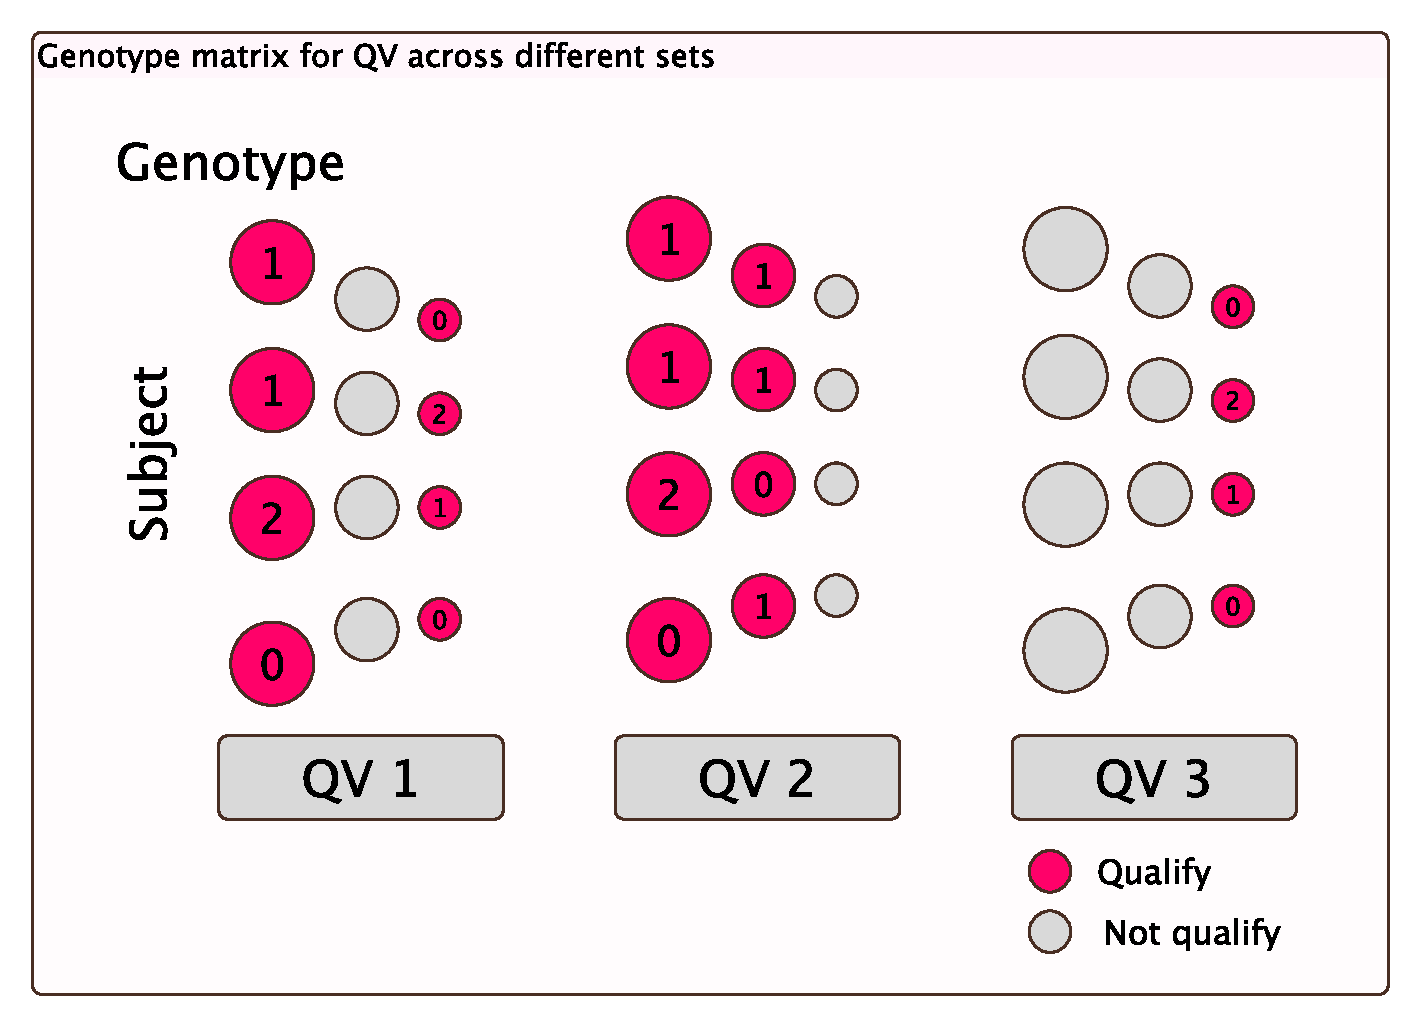
\includegraphics[width=0.99\textwidth]{./images/qv_matrix.pdf}
    \caption{Genotype matrices for three different layers of \ac{qv} analysed in genetic studies. Each matrix represents a specific set, showing the genotypes of three individuals for three SNPs (SNP1, SNP2, SNP3).
    In the \ac{qv}1 layer, SNP1 and SNP3 qualify as a QV (highlighted in red). The genotypes are for \ac{qv} are coded as 0 for homozygous reference, 1 for heterozygous, and 2 for homozygous alternative.
    }
    \label{fig:qv_matrix}
\end{figure}

An example of a multi-part analysis with sets \ac{qv} sets 1, 2, and 3, 
is illustrated in 
\textbf{Figure \ref{fig:qv_matrix}}.
For simplicity, we can assume that each set represents one \ac{gwas}.
The outcomes of each test can subsequently be combined with statistical methods such as the \ac{acat} \cite{liu2019acat, li2020dynamic}.
It becomes possible to aggregate and compare these results from separate tests. 
This process combines p-values across different analyses or variant sets, accounting for the directions and magnitudes of the effects. 
It not only enhances the power to detect significant associations, especially when variants have heterogeneous effects but also simplifies the interpretation of aggregated genomic data. 
By employing \ac{acat}, we can synthesize findings from multiple \ac{qv} filters applied to the same genomic dataset, leading to a more comprehensive understanding of the genetic architecture of traits under study. 
This method is useful in scenarios where variants across different \ac{qv} sets may contribute in varying degrees to the phenotype, allowing for a nuanced analysis that respects the complexity of genomic data.
The combination method must be adapted in scenarios where variants (or collapsed variant sets) do not overlap. 
We have previously provided methods to plot the results of such analysis with \href{https://github.com/DylanLawless/archipelago}{archipelago}  (cite pre-print instead of package).

\subsection{Applications in complex data and multiblock fusion} 

Multiblock data fusion is an emerging yet nascent field in statistics and machine learning  which is championed by multi-omics. 
The interplay between statistical theory and machine learning unveils profound opportunities for advancing our understanding of complex biological systems.
This approach harnesses the power of diverse data types through sophisticated fusion techniques that integrate multiple blocks of omics data - be it DNA, RNA, protein, or clinical data - into a coherent analytical framework. 
Such integration not only enhances the resolution at which we understand disease mechanisms but also refines our predictive capabilities across different scales of biological organisation. 
By applying advanced statistical models 
%Principal Component Analysis, Generalised Canonical Correlation Analysis, and Multiblock Partial Least Squares, 
researchers can uncover nuanced relationships within and between datasets that were previously obscured. 
\citet{kong2018nature} and \citet{howe2021within} have previously shown 
how complex signals can exist within single datasets.

% \cite{kong2018nature} % This paper shows for the first time that part of the signal in the \ac{gwas} for some traits is from ‘indirect genetic effects’ that act through parents rather than directly on the index individual, and shows how these can be disentangled with family data.
% \cite{howe2021within} % This study is the largest within-sibship \ac{gwas} to date and illustrates the value of this method for disentangling direct genetic effects from indirect genetic effects and population structure.

These methods allow for a detailed exploration of how different biological signals interact, offering a richer, more comprehensive view of the genomic landscape. 
As these techniques evolve, they promise to break new ground in predictive modeling and theoretical biology, providing insights that are as profound as they are essential for precision medicine and personalised health interventions.

We contend that the term ``\ac{qv}'', when standardised and optimised for advanced multi-stage use rather than simplistic, single-stage filters, not only advances omics research but also opens up unexplored theoretical domains. 
This includes a multi-dimension analysis of a single data source through exploring new concepts; for example, such jointly analysing probative variants (potentially axiomatically-causal with missing evidence), 
associational, causal, and counterfactual queries, in combination with traditional analyses that integrate other omic markers like RNA and protein abundance.
Sophisticated \ac{qv} applications that combine various sets of \ac{qv}s on a single data source may prepare the correct joint dataset for such complex analyses.
The resulting mixed-up mixed model requires new frameworks.

By deploying a variety of \ac{qv} protocols simultaneously on a single dataset, we orchestrate a multi-dimensional analysis that spans the full spectrum of genomic inquiry. This integrated approach allows for the combination of various \ac{qv} protocols tailored to the specifics of the dataset, engaging different types of data analyses that can range from genetic variations to complex disease markers and beyond. 
The integration of these diverse analytical layers facilitates a comprehensive examination of genetic factors on both individual and cohort levels, promoting understanding that could propel genetic insights. This complex interplay between multiple \ac{qv} sets catalyses the advancement of new theories in multi-omic research.

\subsection{Protocol development and standardisation needs} 

These complex approaches requires a clear protocol for merging data across different layers, ensuring that each contributes meaningfully to the unified model without conflating their distinct signals. 
Therefore, a standardised definition and reporting style for \ac{qv} are crucial for the rapid development of new theories, especially in scenarios where data may not be publicly available, and codebases are complex. 
The nuanced and widespread steps of \ac{qv} across lengthy pipelines will benefit from being reported explicitly as a protocol with a detailed list of definitions and variables, building on our demonstrated examples for one such set, \ac{qv}1.

\section{Future directions and implications} 
\subsection{Integration strategies}
%Discussion on the necessity of sophisticated data integration strategies. Predictions for the future of omics research with the standardized use of refined \ac{qv}s.
We consider the impact of new publishing formats like Registered Reports on the field of genomics, promoting transparency and reproducibility 
\cite{chambers2014instead}. % This paper introduces the Registered Reports concept, a publishing format in which peer review occurs before data collection and analysis. 
% Thinking about the paper: "Instead of" playing the game" it is time to change the rules: Registered Reports at AIMS Neuroscience and beyond" - how we should have something equivalent for \ac{qv} too.
This kind of approach will be crucial as we develop increasingly sophisticated machine learning and artificial intelligence models capable of integrating vast multi-omic datasets. The potential for these models to unravel complex biological phenomena is immense, yet the challenge remains in assembling sufficient training data. Particularly in the realm of rare diseases, the raw data from human cases potentially do not meet the extensive needs of these advanced models. The embeddings or feature representations derived from raw data may be insufficient for training robust models; however, properly formatted and curated \ac{qv}s may enrich these representations, enhancing the potential for accurate model training. If so, the accurate and strategic application of \ac{qv}s becomes essential. By effectively identifying key data through refined \ac{qv} protocols, researchers can enhance the accuracy and efficacy of predictive models, opening up new avenues for significant biological discoveries.

The need for advanced \ac{qv} protocols that can effectively manage such complexity is critical, particularly in the development of statistical methods designed to navigate the intricate relationships within and across diverse omic data blocks. A standardised and nuanced application of \ac{qv}s, detailed through explicit protocols and definitions, is fundamental for the evolution of new analytical frameworks. Therefore, we advocate for a more refined and comprehensive use of \ac{qv}s, advancing beyond traditional single-stage filters to meet the sophisticated demands of modern multi-omic research. 

\subsection{Notation typical to GWAS, VSAT, and other statistical applications}
We explore the notational use of \ac{qv} in commonly used applications to demonstrate how the conceptual framework can accelerate adoption in theoretical domains. 
For example, in GWAS \cite{uffelmann2021genome} the notation for the logistic regression model for estimating the probability of case status is given by:
$$
\text{logit}(p_i) = \log\left(\frac{p_i}{1 - p_i}\right) = \beta_0 + \sum_{k=1}^n \beta_k x_{ik} + \beta_{\text{geno}} G_i
$$
where:
\( p_i \) is the estimated probability that individual \( i \) is a case, based on their genotypic and covariate data,
\( \beta_0 \) is the intercept,
\( \beta_k \) are the coefficients for the covariates,
\( x_{ik} \) represents the covariate values for the \( i \)-th individual,
\( \beta_{\text{geno}} \) is the coefficient for the genetic effect,
\( G_i \) is the genotype of the \( i \)-th individual, coded as 0, 1, or 2  (representing the number of minor alleles).

The following version shows the explicit GWAS model with QV notation:
% $$\text{logit}(p_i) = \log\left(\frac{p_i}{1 - p_i}\right) = \beta_0 + \beta_1 \text{sex}_i + \beta_2 \text{log10(age)}_i + \sum_{j=1}^{10} \beta_{2+j} \text{PC}_j^{(i)} + \beta_{13} G_{\text{QV}_{i,v}}$$

$$
\text{logit}(p_i) = \log\left(\frac{p_i}{1 - p_i}\right) = \beta_0 + \beta_1 \text{sex}_i + \beta_2 \text{log10(age)}_i + \sum_{j=1}^{10} \beta_{2+j} \text{PC}_j^{(i)} + \sum_{k=1}^{n} \beta_{13+k} G_{\text{QV}_{i,v,k}}
$$\\
where:
% \( \beta_0 \) is the intercept,
\( \beta_1 \) adjusts for sex (1 if male, 0 if female),
\( \beta_2 \) adjusts for the log-transformed age in days,
\( \beta_3 \) to \( \beta_{12} \) correspond to the first ten principal components, adjusting for population stratification,
%\( \beta_{13} \) is the effect of the genotype on the phenotype, with \( G_{\text{QV}_{i,v}} \) denoting the genotype of the \( i \)-th individual for the \( v \)-th variant in the QV set.
 \( \beta_{13+k} \) represents the effects of the genotype on the phenotype for each additional qualifying variant set \( k \),
\( G_{\text{QV}_{i,v,k}} \) denotes the genotype of the \( i \)-th individual for the \( v \)-th variant in the \( k \)-th \ac{qv} set.

Likewise, SKAT and its optimal unified version, SKAT-O, are now popular methods for gene-based association tests that accommodate multiple variants within a gene or variant set while accounting for their potentially differing directions and magnitudes of effects
\cite{wu2011rare, lee2012optimal}. 
The logistic regression model for SKAT, taking into account the specific variants from the QV set, can be described as follows:
$$
\log \left( \frac{P}{1-P} \right) = X_i \gamma + G_{\text{QV}_{i,v}} \beta
$$
where:
\( P \) is the disease probability,
\( \gamma \) is an \( s \times 1 \) vector of regression coefficients of covariates,
\( \beta \) is an \( m \times 1 \) vector of regression coefficients for genetic variants,
\( G_{\text{QV}_{i,v}} \) denotes the genotype values for all variants \( v \) in the QV set for individual \( i \).
The SKAT statistic is then:
$$
Q_S = (y - \hat{\pi})^\top K (y - \hat{\pi})
$$
where \( \hat{\pi} \) is the vector of the estimated probability of \( y \) under the null model, and \( K \) is the kernel matrix defined as \( G_{\text{QV}} W G_{\text{QV}}^\top \), with \( W \) being the diagonal weight matrix for the variants.

With these familiar examples established, we can consider more complex models where other variants outside of the main \ac{qv} set can be assessed,  $QV_{1,...,n} $,
which we describe in the next section. 
These sets can represent different categorisations or stratifications of genetic variants that might be relevant under varying analytical conditions or specific studies.

\subsection{Conceptual framework and statistical representation}

In \ac{gwas}, the transition from empirically testable variants (\ac{qv}1) to theoretical \ac{ax} marks a pivotal stage in genetic research.
\ac{ax} comprises genetic variants that ideally conform to fundamental genetic principles and are thus considered correct by genetic doctrine. 
However, due to technological constraints and gaps in genetic understanding, \ac{ax} remains largely theoretical and unverifiable empirically. 
In contrast, \ac{qv}1 includes those variants from \ac{ax} that survive rigorous empirical filtering, applying standard \ac{gwas} pre-processing criteria such as --geno, --maf, --hwe, and --mind, aimed at ensuring the quality and relevance of data by removing variants based on missing genotype data, minor allele frequency, Hardy-Weinberg equilibrium deviations, and individual missing data thresholds.

It is important to emphasise the distinction we are considering: we are dealing with unobserved or unknown variants, rather than variants of unknown significance, in the Bayesian sense.
The mathematical representation of the relationship between \ac{ax} and \ac{qv}1 is crucial for understanding the impact of this transition. Firstly, the intersection operation:
$$
\text{TP} = QV\textsubscript{ax} \cap QV1,
$$
identifies true positive variants, which are both theoretically ideal and empirically robust, thus successfully passing the \ac{gwas} filtering criteria.
 Secondly, the set difference operation:
$$
\text{FN} = QV\textsubscript{ax} \setminus QV1,
$$
calculates false negatives, representing the axiomatic variants that were erroneously excluded by the empirical filters, potentially omitting key genetic signals. 
Lastly, the quantification of unknowns:
$$
\text{Unknowns} = |QV\textsubscript{ax}| - |\text{TP}|,
$$
provides a measure of the magnitude of theoretical variants that remain untested or unconfirmed after processing, emphasizing the potential loss of valuable genetic information.

This structured approach not only clarifies the dynamics between the axiomatic and filtered variants but also underscores the trade-offs involved in \ac{wgs} pre-processing. 
By balancing data quality against the risk of overlooking significant genetic contributors, this analytical framework aids us in navigating the complexities of genetic data preparation and evaluation.

We explore these applications in detail elsewhere (cite Bayesian framework paper), but we briefly summarise the ideas here. 
% \subsection*{Estimating Unknowns with Bayesian Statistics}
In the context of \ac{gwas}, Bayesian statistics offers a potent framework for integrating theoretical and empirical knowledge. 
This approach leverages prior biochemical and genetic data to refine our understanding of the landscape of genetic variants, particularly those beyond current empirical capabilities.

% \subsubsection*{Bayesian Framework}
We start by defining a prior distribution \( P(\theta) \) based on established knowledge about DNA mutation rates and variant frequencies, reflecting our initial beliefs about the genetic variant distribution. Given a dataset \( D \) from GWAS pre-processing (QV1), the likelihood function \( P(D|\theta) \) assesses the probability of observing the data under various genetic configurations dictated by \( \theta \).

The \textbf{posterior distribution} \( P(\theta|D) \), derived from Bayes' theorem,
$$P(\theta|D) = \frac{P(D|\theta) \times P(\theta)}{P(D)},$$
where \( P(D) \) serves as a normalizing constant, updates our beliefs in light of new data. This posterior distribution integrates both the prior information and the empirical data from GWAS, providing a nuanced estimate of the distribution of genetic variants.
%\subsubsection*{Quantification of Unknowns}
The ``unknowns'' in our study, representing genetic variants not observed but theoretically possible within QV\_ax, are quantified as follows:
$$
\text{Unknowns} = \int_{\theta \in \Theta_{\text{unobserved}}} P(\theta|D) \, d\theta,
$$
where \( \Theta_{\text{unobserved}} \) encompasses all parameter values corresponding to unobserved variants. 
This integral effectively measures the total probability of variants that are conceivable but not detected in the empirical dataset \ac{qv}1.

With this short demonstration of potential future directions, we conclude our exploration of the methodological framework and practical applications.

\section{Enhancing semantic interoperability}
The Swiss Personalized Health Network (SPHN) promotes data sharing based on the FAIR principles, supported through the SPHN RDF Schema to enhance semantic interoperability, particularly for clinical routine data
\cite{wilkinson2016fair}. 
The recent extension of this schema incorporates genomic data processing, enriching it with detailed genomic-specific concepts that span from sample processing to the sequencing run \cite{van2023bridging}.
This extension includes critical concepts such as the sequencing instrument and \ac{qc} metrics, which are necessary in ensuring the integrity and reproducibility of genomic analyses. To further integrate omics data within clinical frameworks, we have developed additional concepts, such as omic analysis results, that enable the reporting of outcomes directly tied to clinical care.

The \ac{qv} framework allows for the explicit recording of \ac{qv} sets used in analyses. 
This is particularly beneficial as it provides a robust mechanism to track and verify the application of specific variant sets, such as those defined by the \ac{acmg} \ac{sf}, independent of internal protocol changes. 
Such a feature ensures that users can query and confirm the use of specific \ac{qv} sets, like the \ac{acmg} \ac{sf}, without the need to delve into the specifics of source protocols. 
This not only streamlines the verification process but also enhances the transparency and traceability of genomic analyses within the SPHN framework.

Therefore, to enhance reproducibility and traceability in omics research, we propose the \ac{qv} Set ID (\texttt{qualifying\_variant\_set\_id} ). This identifier crucially links the variant sets used in analyses, facilitating precise and consistent replication of research methodologies.
Implementing unique identifiers for qualifying variant sets is essential to ensure the reproducibility of omics analyses. These identifiers must be unique, consistent, and align with existing data management standards, integrating seamlessly into RDF schemas that incorporate standards like SNOMED CT.

As a community, we have yet to agree on the consensus sharing method. 
We provide several examples for generating unique identifiers:

\begin{enumerate}
    \item \textbf{Hash functions:} SHA-256 to generate a unique hash of the set's characteristics, ensuring a unique and reliable identifier.
    \item \textbf{UUIDs:} Employ randomly generated UUIDs which provide high uniqueness across systems.
    \item \textbf{Semantic combination:} Create identifiers by combining relevant semantic elements like project ID and data release version in a structured format.
    \item \textbf{IRI incorporation:} Develop internationalised resource identifiers (IRI) that provide traceability and integrate neatly into linked data frameworks.
    \item \textbf{Registry-based allocation:} Use a centralised registry to manage identifier assignment and ensure consistency.
    \item \textbf{Integrating standards:} Use standards such as SNOMED CT with local identifiers to form comprehensive, domain-specific identifiers.
\end{enumerate}

We demonstrate an example analysis plan (or result database entry) in \textbf{box \ref{box:example_concept}}. 
This lists the pipeline used, three hypothetical internal \ac{qv} sets (\texttt{qv1, qv2, qv3}) and one well-known public shared \ac{qv} set \texttt{acmg\_sf\_v3.2}  where the sha256 can be confirmed.
Anyone reviewing the analysis results can be sure that \ac{qv} criteria \texttt{acmg\_sf\_v3.2} has been included in the protocol.

\begin{tcolorbox}[
    % breakable,  % Allows the box to split over pages
    colback=white!0,  % No background color (fully transparent)
    colframe=black,  % Black border color
    boxrule=1pt,  % Width of the border
    arc=1mm,  % Radius of the corner rounding
    outer arc=1mm,
%    title=\textbf{Example diagrammatic representation}
   title=\textbf{\refstepcounter{myboxcounter}\label{box:example_concept}Box \themyboxcounter: Example implementation}
]

pipeline: \colorbox{colorSUNSET1!30}{\texttt{pipeline DNA SNV INDEL v1}}\\
qualifying\_variant\_set\_id: \colorbox{colorSUNSET2!60}{\texttt{qv1\_20250201.yaml}}\\
qualifying\_variant\_set\_id: \colorbox{colorSUNSET2!60}{\texttt{qv2\_20250201.yaml}}\\
qualifying\_variant\_set\_id: \colorbox{colorSUNSET2!60}{\texttt{qv3\_20250201.yaml}}\\
qualifying\_variant\_set\_id: \colorbox{colorSUNSET2!60}{\texttt{acmg\_sf\_v3.2}}\\

where 
\begin{verbatim}
$ shasum -a 256 acmg_sf_v3.2.tsv | fold -w 32
6ad26a7df2feda3e2d4bfabf4a3cb1ca
4356b098ccc0890a7a17f198a9ab117f
acmg_sf_v3.2.tsv
\end{verbatim}
\end{tcolorbox}

Incorporating \texttt{qualifying\_variant\_set\_id} not only enhances transparency but also increases operational efficiency in omics data handling, facilitating precise and reproducible research across various projects.

\section{Validation case study}

We demonstrate that 100\% of criteria were correctly applied using the standardised \ac{qv} criteria compared with the typical manual version in our case study example.
In this process we applied an \ac{acmg} variant classification
protocol \cite{richards2015standards} using a standardised \ac{qv} criteria in YAML format.
We used a rare disease cohort of 940 individuals, pre-processed for 
\ac{qc} and a minimal \ac{qv} test set, as previously described (lawless spss 2025). 
For ease of reporting, this example was restricted to chromosome 1, which contained 596 qualifying variants after strict filtering (MAF < 0.01) and limited to known disease genes based on the Genomics England panel ``Primary immunodeficiency or monogenic inflammatory bowel disease,'' retrieved using our PanelAppRex R repository (\href{https://github.com/DylanLawless/PanelAppRex}{GitHub link}). 
We prepared this annotation interpretation dataset in R with GuRu, our variant interpretation tool, which consolidates all annotation sources and scores variants. The annotated dataset was imported from gVCF format (output by VEP) and stored as a table of 596 variant rows with 377 annotation columns. A brief selection of the annotations used used for \ac{qv} is shown in \textbf{figure \ref{fig:guru_case_study_setup}}.

\begin{figure}[!h]
    \centering
   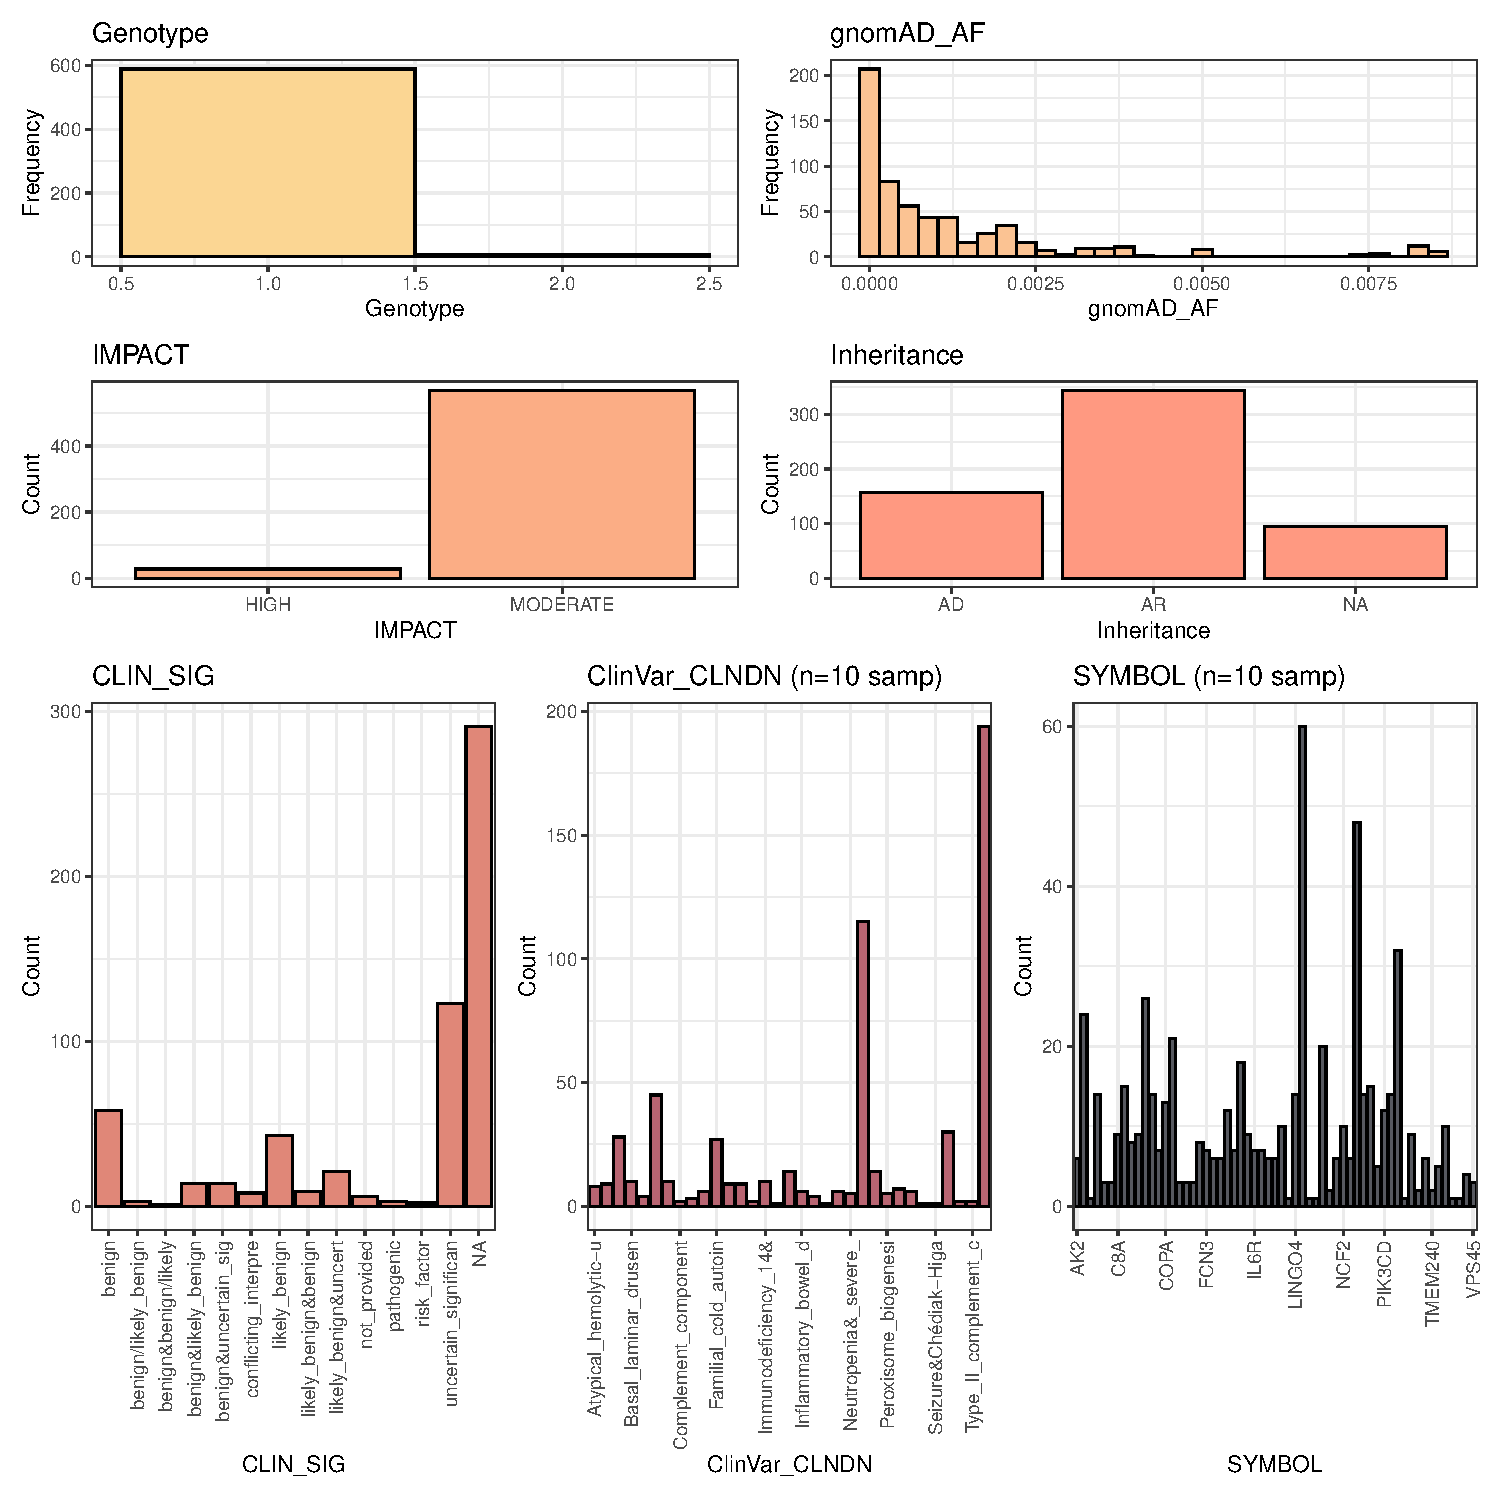
\includegraphics[width=0.85\textwidth]{./images/Guru_singlecase_distribution_variables.pdf}
       \caption{Example of the annotated dataset describing variant calls from the disease cohort on chromosome 1. The subset shown highlights key variables used in quality control and variant interpretation, resulting in 596 variants with 377 annotation fields per variant for 940 subjects. Axis which contain many term labels are down sampled to list every tenth  label (n=10 samp).}
    \label{fig:guru_case_study_setup}
\end{figure}

We selected the first eight ACMG criteria for assigning pathogenicity scores to variants \cite{richards2015standards}. Of these eight, six were relevant for the cohort.
First, we performed this analysis manually by hard coding each criterion in the script, reflecting a typical analysis scenario. Second, we imported the same criteria from the \ac{qc} YAML file to represent our standardised approach. We captured the outputs from both scoring methods and compared them, as shown in \textbf{figure \ref{fig:guru_case_study_result}}.
The \ac{qv} criteria in YAML format are found in file \texttt{qv\_files/acmg\_criteria.yaml} and are in the following style in 
\textbf{box \ref{box:acmg_criteria_yaml}}:

\begin{tcolorbox}[
    % breakable,  % Allows the box to split over pages
    colback=white!0,  % No background color (fully transparent)
    colframe=black,  % Black border color
    boxrule=1pt,  % Width of the border
    arc=1mm,  % Radius of the corner rounding
    outer arc=1mm,
%    title=\textbf{Example diagrammatic representation}
   title=\textbf{\refstepcounter{myboxcounter}\label{box:acmg_criteria_yaml}Box \themyboxcounter: qv\_files/acmg\_criteria.yaml}
]

\begin{verbatim}
ACMG_PVS1:
  description: >
    Null variants (IMPACT = HIGH) in genes where 
    loss-of-function causes disease.
    Includes homozygous variants, dominant inheritance, 
    and compound heterozygous cases.
    Compound heterozygosity is considered when both 
    variants are HIGH impact. WARNING: Not phase checked.
  logic: "or"
  conditions:
    - condition:
        field: IMPACT
        value: "HIGH"
        operator: "=="
...
shasum -a 256 acmg_criteria.yaml | fold -w 32
d91fde41a5fff48631adecba38773d61
9ae8cd5cff9b9b42ef7f5efbd6bbfcdf
acmg_criteria.yaml
\end{verbatim}
\end{tcolorbox}


\begin{figure}[!h]
\centering
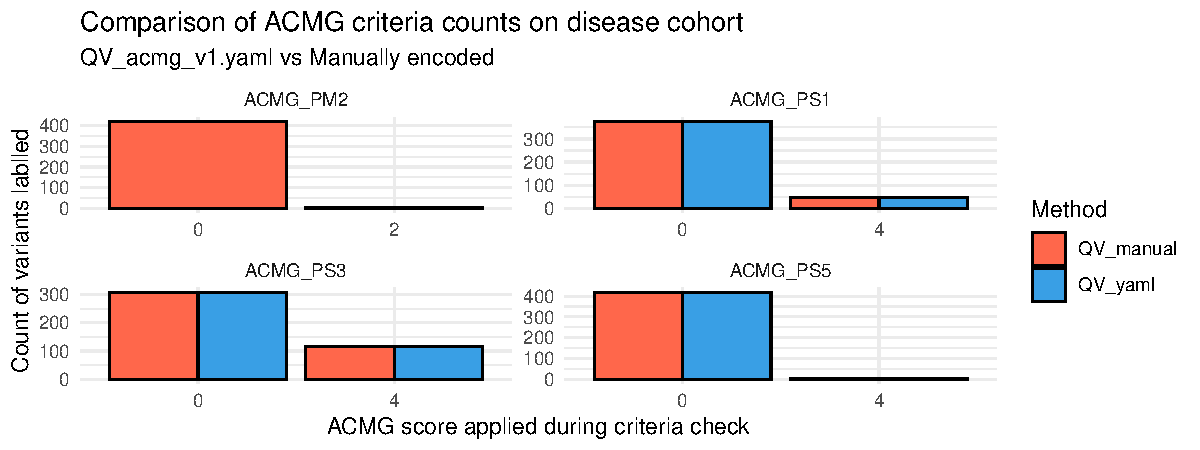
\includegraphics[width=0.99\textwidth]{./images/Guru_singlecase_validation_of_yaml_vs_manual.pdf}
\caption{GuRu case study with an ACMG criteria subset, showing a 100\% match between manually encoded and YAML-based methods (\texttt{qv\_files/acmg\_criteria.yaml}) for assigning pathogenicity scores.}
\label{fig:guru_case_study_result}
\end{figure}

Our results, presented in \textbf{figure \ref{fig:guru_case_study_result}}, show a 100\% match between the two methods, demonstrating that the criteria can be imported from YAML and applied programmatically to achieve the same outcome. This is not necessarily surprising, as the burden of accuracy remains in the implementation. However, the \ac{qc} YAML file acts as a shareable, standalone resource that can be adapted for different pipelines or programming languages, ensuring reproducibility for \ac{qv} criteria.

The YAML criteria used here include \texttt{ACMG\_PS1}, described as``the same amino acid change was a previously established pathogenic variant regardless of nucleotide change.'' It includes \texttt{terms} containing ``pathogenic,'' applies to the \texttt{CLIN\_SIG} (clinical significance) annotation field, and uses ``or'' logic. We also included \texttt{ACMG\_PS3}, which describes well-established functional studies supporting a damaging effect on the gene product, with a user-defined inheritance pattern matching the genotype, and \texttt{ACMG\_PS5}, which covers compound heterozygosity with at least one high-impact variant (according to Ensembl VEP definitions). The \texttt{ACMG\_PM2} criterion states that the variant is absent from controls or present at extremely low frequency in gnomAD or other population databases. For \texttt{ACMG\_PM3}, the criterion checks for variants in trans with a pathogenic variant in recessive disorders, showing some overlap with PS5 because our rare disease cohort filtering already treats ``IMPACT = HIGH'' as pathogenic.

We skipped the PS2 criterion, which requires confirmed de novo status in a patient with the disease and no family history, because no parental data were available. We also skipped PS4, which measures a significantly increased prevalence in affected individuals compared with controls, because that was evaluated in a separate case-control analysis for this cohort.

Subsequently, we briefly demonstrate why such \ac{qv} criteria are necessary. In \textbf{figure \ref{fig:guru_case_study_guruscores}}, we show the final annotation results for the test disease cohort by listing the number of criteria applied for both samples (cases) and variants. From this, the top candidate causal pathogenic variants can be automatically retrieved using ACMG scoring methods \cite{richards2015standards, tavtigian2020fitting}.

\begin{figure}[!h]
\centering
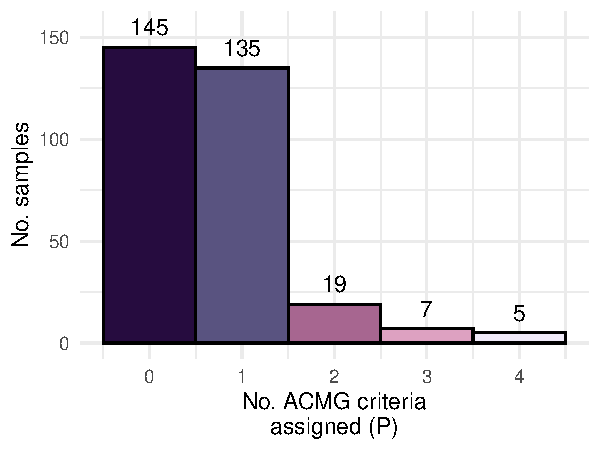
\includegraphics[width=0.49\textwidth]{./images/Guru_singlecase_criteria_per_sample_small.pdf}
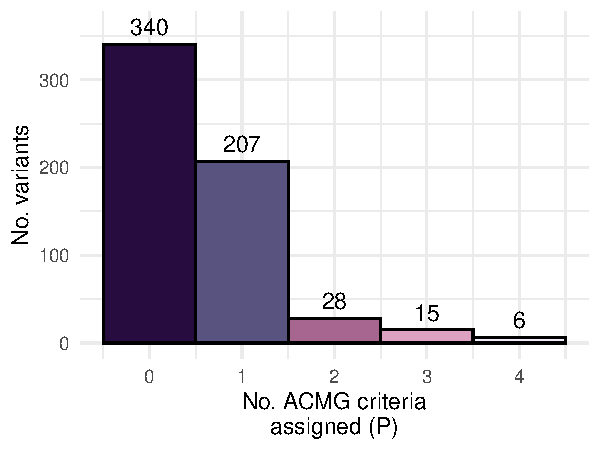
\includegraphics[width=0.49\textwidth]{./images/Guru_singlecase_variants_per_criteria_small.pdf}
\caption{Overview of the final annotation interpretation for the test disease cohort, illustrating the number of criteria applied both for subject samples (left) and for variants (right). This facilitates subsequent retrieval of the top candidate pathogenic variants automatically.}
\label{fig:guru_case_study_guruscores}
\end{figure}

%> print(validation_combined)
%   Var1 Count Criterion    method
%1     0   589 ACMG_PVS1   QV_yaml
%2     8     7 ACMG_PVS1   QV_yaml
%3     0   562  ACMG_PS1   QV_yaml
%4     4    34  ACMG_PS1   QV_yaml
%5     0   435  ACMG_PS3   QV_yaml
%6     4   161  ACMG_PS3   QV_yaml
%7     0   584  ACMG_PS5   QV_yaml
%8     4    12  ACMG_PS5   QV_yaml
%9     0   591  ACMG_PM2   QV_yaml
%10    2     5  ACMG_PM2   QV_yaml
%11    0   570  ACMG_PM3   QV_yaml
%12    2    26  ACMG_PM3   QV_yaml
%13    0   589 ACMG_PVS1 QV_manual
%14    8     7 ACMG_PVS1 QV_manual
%15    0   562  ACMG_PS1 QV_manual
%16    4    34  ACMG_PS1 QV_manual
%17    0   435  ACMG_PS3 QV_manual
%18    4   161  ACMG_PS3 QV_manual
%19    0   584  ACMG_PS5 QV_manual
%20    4    12  ACMG_PS5 QV_manual
%21    0   591  ACMG_PM2 QV_manual
%22    2     5  ACMG_PM2 QV_manual
%23    0   570  ACMG_PM3 QV_manual
%24    2    26  ACMG_PM3 QV_manual
%> print(dim(df))
%[1] 596 377

\section{Conclusions}
We emphasise the critical importance of \ac{qv} standardisation in genomic research. By proposing a clear framework for incorporating \ac{qv} protocols into analysis pipelines, we highlight how systematic handling of these variables enhances reproducibility, accuracy, and efficiency in genetic studies. As genomic technologies and data complexities expand, the need for robust, scalable, and adaptable \ac{qv} protocols becomes ever more pressing. Future work should extend these frameworks to accommodate emerging technologies and analytical challenges, further improving the fidelity and utility of genomic data interpretation across diverse applications.

\clearpage
\bibliographystyle{unsrtnat}
\bibliography{references}  %%% Uncomment this line and comment out the ``thebibliography'' section below to use the external .bib file (using bibtex) .

%
%\section{Supplemental}
%
%The VQSR example is shown in the format of a workflow manager:
%
%\begin{tcolorbox}[
%    breakable,  % Allows the box to split over pages
%    colback=white!0,  % No background color (fully transparent)
%    colframe=black,  % Black border color
%    boxrule=1pt,  % Width of the border
%    arc=1mm,  % Radius of the corner rounding
%    outer arc=1mm,
%    title=\textbf{\refstepcounter{myboxcounter}\label{box:vqsr_example}Box \themyboxcounter: Variant Quality Score Recalibration (VQSR) in Snakemake}
%]
%\begin{verbatim}
%# Snakefile for VQSR
%configfile: "config.yaml"
%qv_settings = read_yaml(config["qv_config"])
%
%rule all:
%  input:
%    "results/recalibrated_snps.vcf"
%
%rule vqsr_recalibrate_snps:
%  input:
%    vcf="data/raw_snps.vcf"
%  output:
%    recal="results/recalibrated_snps.vcf",
%    tranches="results/snps.tranches"
%  params:
%    ref=config['reference_genome'],
%    hapmap=qv_settings['vqsr_snp_hapmap'],
%    omni=qv_settings['vqsr_snp_omni'],
%    thousandG=qv_settings['vqsr_snp_1000g'],
%    java_opts="-Xmx4g"
%  shell:
%    """
%    gatk --java-options "{params.java_opts}" VariantRecalibrator \
%    -R {params.ref} \
%    -V {input.vcf} \
%    --resource:hapmap,known=false,training=true,truth=true,prior=15.0 {params.hapmap} \
%    --resource:omni,known=false,training=true,truth=false,prior=12.0 {params.omni} \
%    --resource:1000G,known=false,training=true,truth=false,prior=10.0 {params.thousandG} \
%    -an QD -an MQ -an MQRankSum -an ReadPosRankSum -an FS -an SOR \
%    --mode SNP \
%    -O {output.recal} \
%    --tranches-file {output.tranches}
%    """
%\end{verbatim}
%\end{tcolorbox}




\end{document}
